% VUT FIT MITAI
% MSZ 2021/2022
% Author: Vladimir Dusek
% Login: xdusek27

%%%%%%%%%%%%%%%%%%%%%%%%%%%%%%%%%%%%%%%%%%%%%%%%%%%%%%%%%%%%%%%%%%%%%%%%%%%%%%%%

% Path to figures
\graphicspath{{gal/hledani_minimalni_kostry/figures}}

%%%%%%%%%%%%%%%%%%%%%%%%%%%%%%%%%%%%%%%%%%%%%%%%%%%%%%%%%%%%%%%%%%%%%%%%%%%%%%%%

\chapter{GAL -- Hledání minimální kostry obyčejného grafu (pojmy, stromy a kostry, Kruskalův algoritmus, Primův algoritmus).}

%%%%%%%%%%%%%%%%%%%%%%%%%%%%%%%%%%%%%%%%%%%%%%%%%%%%%%%%%%%%%%%%%%%%%%%%%%%%%%%%

\section{Metadata}

\begin{compactitem}
    \item Předmět: Grafové algoritmy (GAL)
    \item Přednáška:
    \begin{compactitem}
        \item 5) Stromy, minimální kostry, Jarníkův a Borůvkův algoritmus.
        \item 6) Růst minimální kostry, algoritmy Kruskala a Prima.
    \end{compactitem}
    \item Záznam:
    \begin{compactitem}
        \item 2020-10-22
        \item 2020-10-29
    \end{compactitem}
\end{compactitem}

%%%%%%%%%%%%%%%%%%%%%%%%%%%%%%%%%%%%%%%%%%%%%%%%%%%%%%%%%%%%%%%%%%%%%%%%%%%%%%%%

\section{Úvod a kontext}

\paragraph*{Orientovaný graf} Orientovaný graf je dvojice $G = (V, E)$, kde $V$ je konečná množina uzlů a $E \subseteq V \times V$ je množina hran.

\paragraph*{Neorientovaný graf} Neorientovaný graf je dvojice $G = (V, E)$, kde $V$ je konečná množina uzlů a $E \subseteq \binom{V}{2}$ je množina hran. (Hrana je tedy dvouprvková množina, avšak běžně se držíme stejného značení jako u~orientovaných grafů a používáme dvojici.)

\paragraph*{Ohodnocený graf} Ohodnocený graf je takový graf, jehož každá hrana má přiřazenou nějakou hodnotu, typicky definovanou pomocí váhové funkce $w : E \mapsto \mathbb{R}$.

\paragraph*{Podgraf} Graf $G' = (V', E')$ je podgraf grafu $G = (V, E)$ jestliže $V' \subseteq V$ a $E' \subseteq E$.

\paragraph*{Sled} Posloupnost uzlů $\langle v_0, v_1, \dots, v_k \rangle$, kde $(v_{i-1}, v_i) \in E$ pro $i = 1, \dots, k$ se nazývá sled délky $k$ z~$v_0$ do $v_k$.

\paragraph*{Uzavřený sled} Sled $\langle v_0, v_1, \dots, v_k \rangle$ se nazývá uzavřený, pokud existuje hrana $(v_0, v_k)$.

\paragraph*{Dosažitelnost} Pokud existuje sled $s$ z~uzlu $u$ do uzlu $v$, říkáme, že $v$ je dosažitelný z~$u$ sledem $s$, značeno $u \xRightarrow{\text{s}} v$.

\paragraph*{Tah} Tah je sled ve kterém se neopakují hrany.

\paragraph*{Cesta} Cesta je sled ve kterém se neopakují uzly.

\paragraph*{Souvislý graf} Neorientovaný graf se nazývá souvislý, pokud mezi libovolnými dvěma uzly existuje cesta.

\paragraph*{Kružnice} Uzavřená cesta se nazývá kružnice.

\paragraph*{Cyklus} Orientovaná kružnice se nazývá cyklus (první a poslední uzel je shodný).

\paragraph*{Prostý graf} Orientovaný graf bez cyklů se nazývá prostý.

\paragraph*{Acyklický graf} Graf je bez cyklů, resp. kružnic, se nazývá acyklický.

\paragraph*{Strom} Graf, který je souvislý a acyklický, se nazývá strom.

\paragraph*{Kostra} Strom, který tvoří podgraf souvislého grafu na množině všech jeho vrcholů, se nazývá kostra (\textit{spanning tree}).

\paragraph*{Minimální kostra} Nechť $G = (V, E)$ je souvislý neorientovaný graf s~váhovou funkcí $w : E \mapsto \mathbb{R}$. Minimální kostra (\textit{MST, minimum spanning tree}) je strom $G' = (V, E')$, kde $E' \subseteq E$ a $$w(E') = \sum_{(u,v) \in T} w(u, v)$$ je minimální ze všech možných alternativních koster.

\paragraph*{Seznam sousedů} Seznam sousedů (\textit{Adj}, \textit{adjacency list}) je reprezentace grafu v~paměti. Jde o~preferovanou variantu pro řídké grafy~--~kde $m << n^2$. Pro každý uzel máme definovaný seznam jeho sousedů.

\paragraph*{Matice sousednosti} Matice sousednosti (\textit{adjacency matrix}) je reprezentace grafu v~paměti. Jde o~preferovanou variantu pro husté grafy~--~kde $m$ je skoro $n^2$.

\begin{figure}[H]
    \centering
    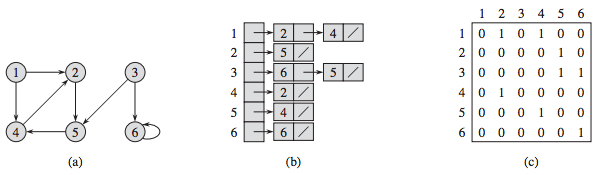
\includegraphics[width=1\linewidth]{graph_representations_example.png}
    \caption{Příklad reprezentace grafu pomocí seznamu sousedů a matice sousednosti.}
\end{figure}

%%%%%%%%%%%%%%%%%%%%%%%%%%%%%%%%%%%%%%%%%%%%%%%%%%%%%%%%%%%%%%%%%%%%%%%%%%%%%%%%

\section{Generický algoritmus}

Hledání minimální kostry je problém, který lze řešit algoritmy, které spadají do kategorie tzv. hladových (\textit{greedy}) deterministických algoritmů. Spočívají v~tom, že průběžně odhadují kostru přidáváním dalších hran a nikdy se nemusejí vracet (neprovádí se \textit{backtracking}). Generický algoritmus tvoří jakousi základní kostru pro další, už konkrétní, algoritmy.

\paragraph*{Řez} Nechť $G = (V, E)$ je graf. Řez grafu $G$ je dvojice $(S, V - S)$, kde $\emptyset \subseteq S \subseteq V$.

\paragraph*{Křížení} Hrana $(u, v) \in E$ kříží řez $(S, V - S)$, pokud jeden její konec je v~$S$ a druhý v~$V - S$.

\paragraph*{Respektování} Nechť $A \subseteq E$ je množina hran. Řez $(S, V - S)$ respektuje množinu hran $A$, pokud žádná hrana v~$A$ nekříží řez $(S, V - S)$.

\paragraph*{Lehkost} Nechť $(S, V - S)$ je řez a $B$ je množina hran, která ho kříží. Hrana z~množiny $B$ s~nejmenší hodnotou se nazývá lehká.

\paragraph*{Bezpečnost} Nechť $G = (V, E)$ je souvislý neorientovaný graf s~reálnou váhovou funkcí $w$. Nechť $A \subseteq E$ je součástí nějaké minimální kostry $G$. Nechť $(S, V - S)$ je řez, který respektuje $A$. Nechť $(u, v)$ je lehká hrana křížící $(S, V - S)$. Pak hrana $(u, v)$ je bezpečná pro $A$.

\bigskip\noindent\begin{minipage}{\linewidth}
\begin{lstlisting}[language=Python, caption={Generický algoritmus. Před každou iterací algoritmu je množina $A$ podmnožinou nějaké minimální kostry. Hrana $(u,v) \in E$ je bezpečná pro $A$, pokud $A \cup \{(u, v)\}$ je podmnožinou nějaké minimální kostry.}]
def generic_mst(G):
    # G je graf
    A = {} # A je mnozina hran rozpracovane minimalni kostry
    while netvori_kostru(A, G):
        for hrana in G.E:
            if je_bezpecna(A, hrana):
                A += {hrana}
    return A
\end{lstlisting}
\end{minipage}

\begin{figure}[H]
    \centering
    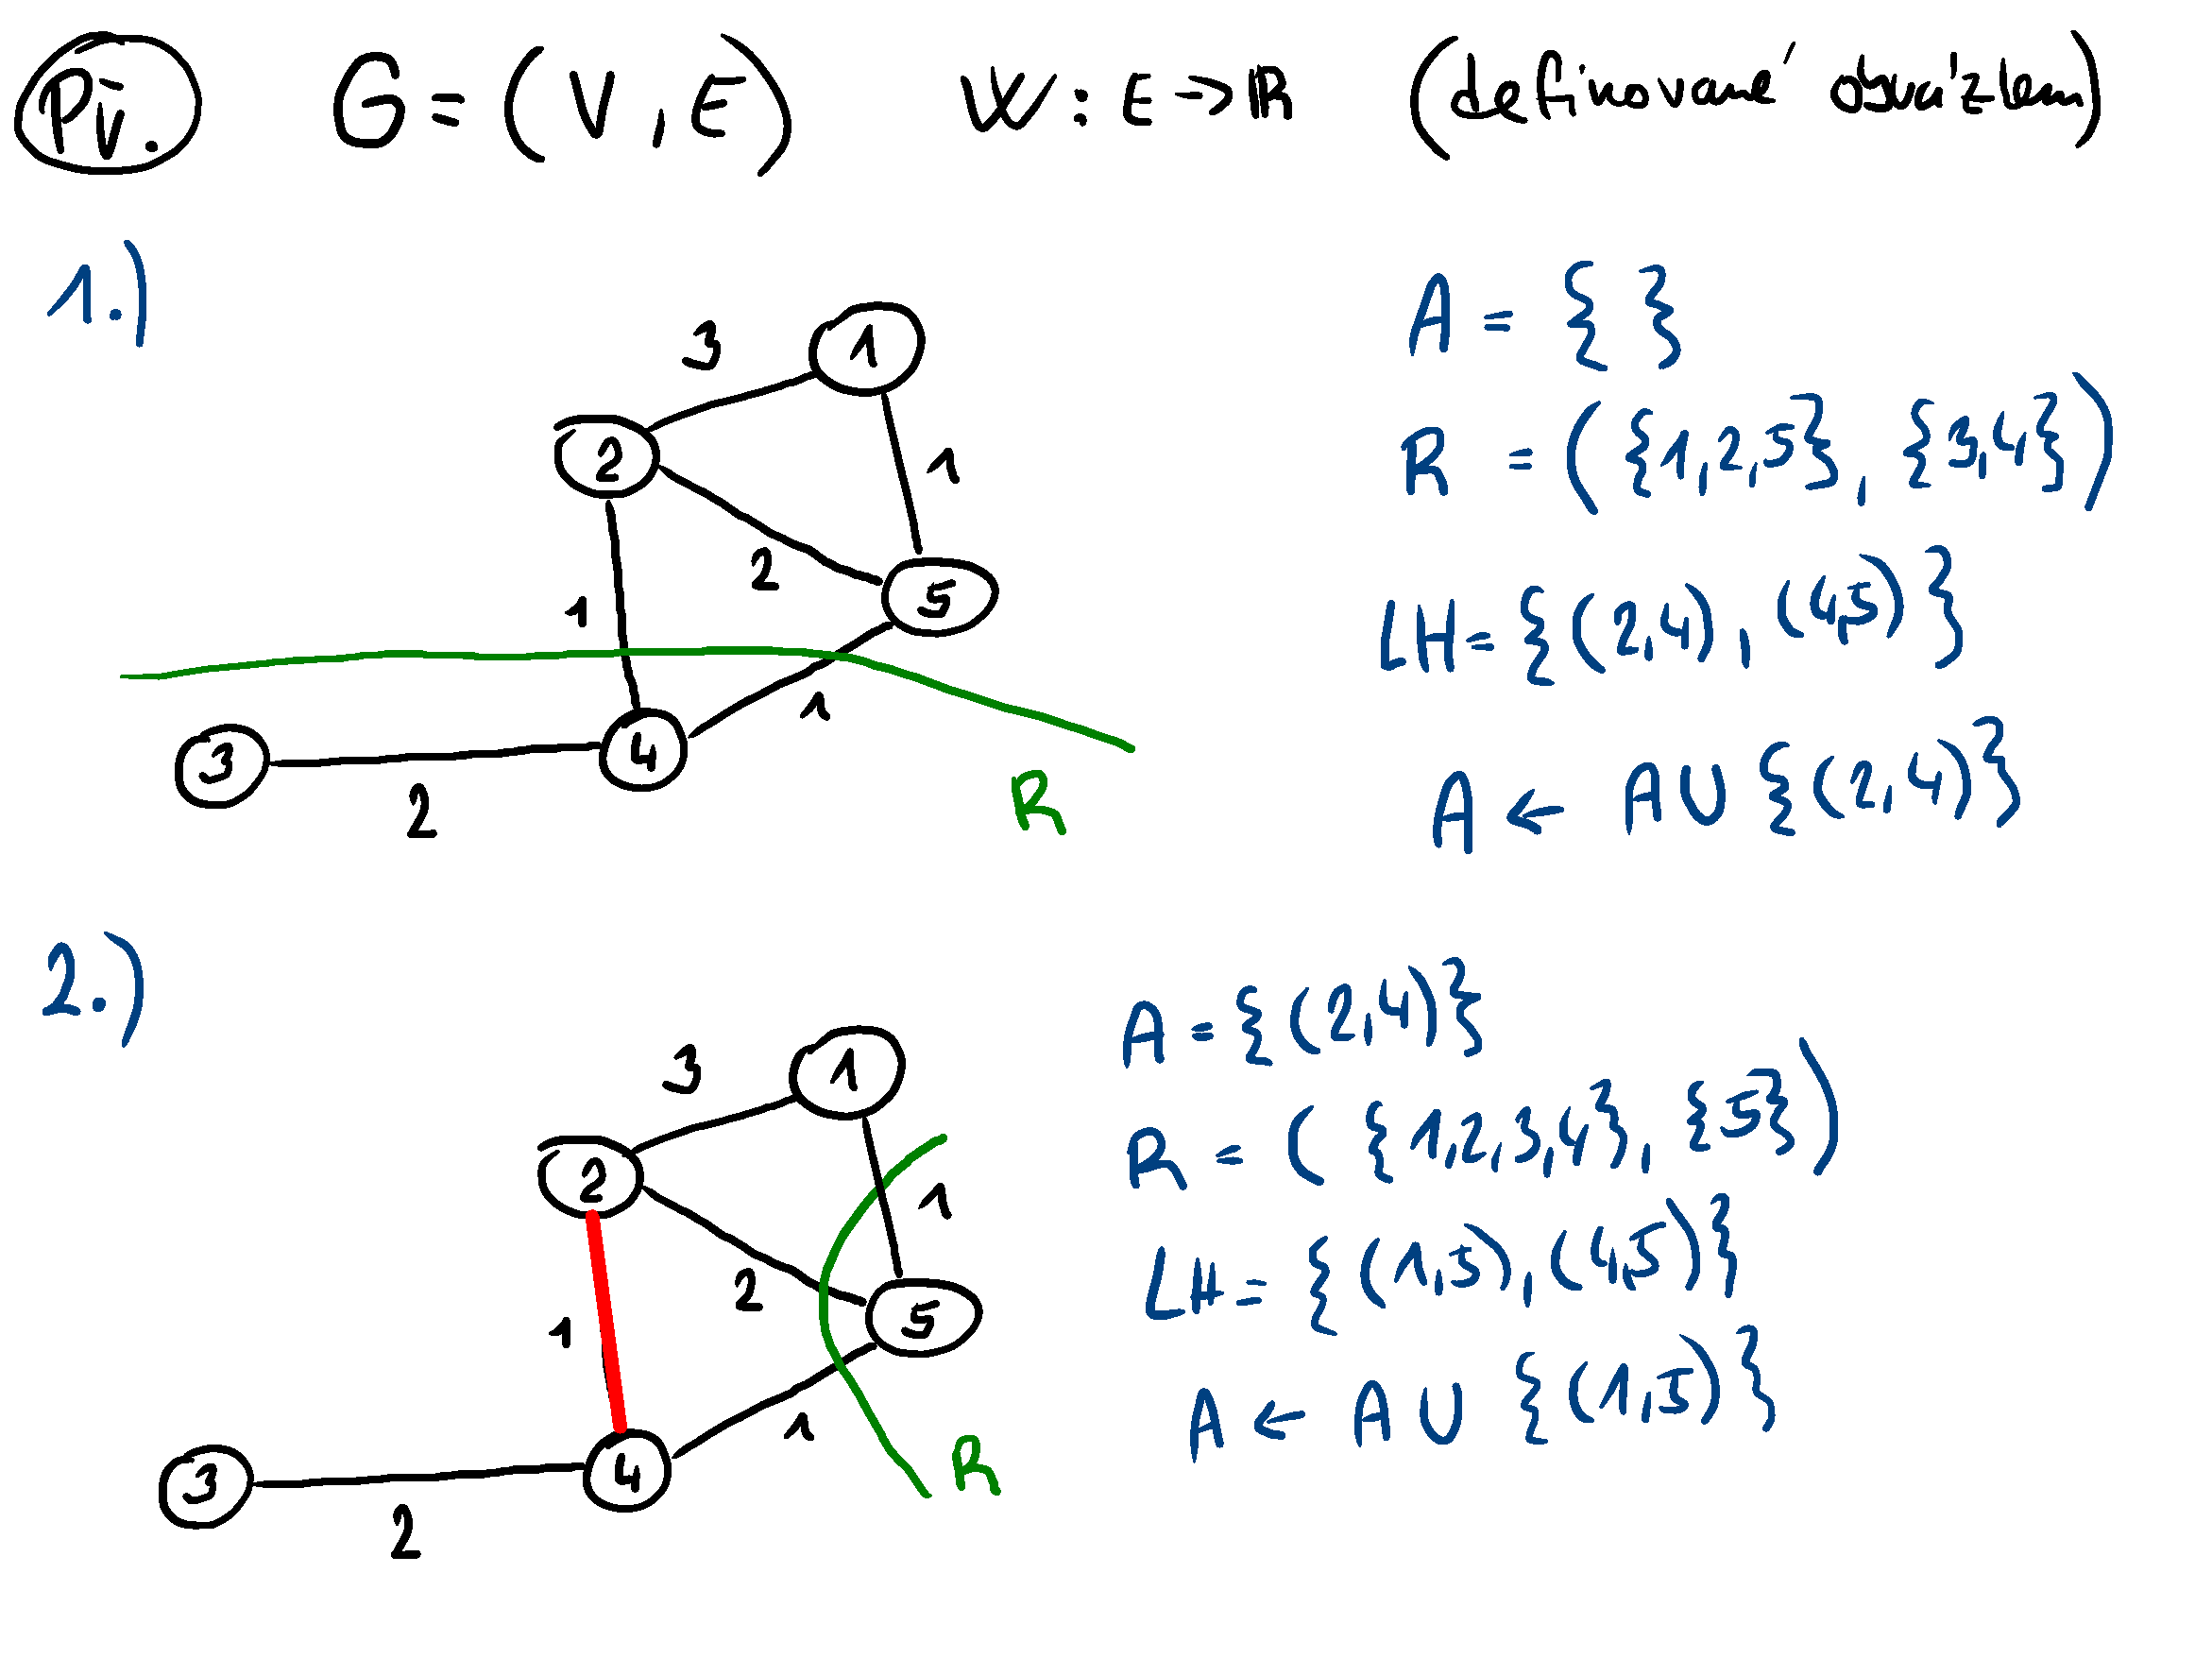
\includegraphics[width=0.9\linewidth]{03-minimalni-kostry-6.pdf}
    \caption{Příklad, část 1.}
\end{figure}

\begin{figure}[H]
    \centering
    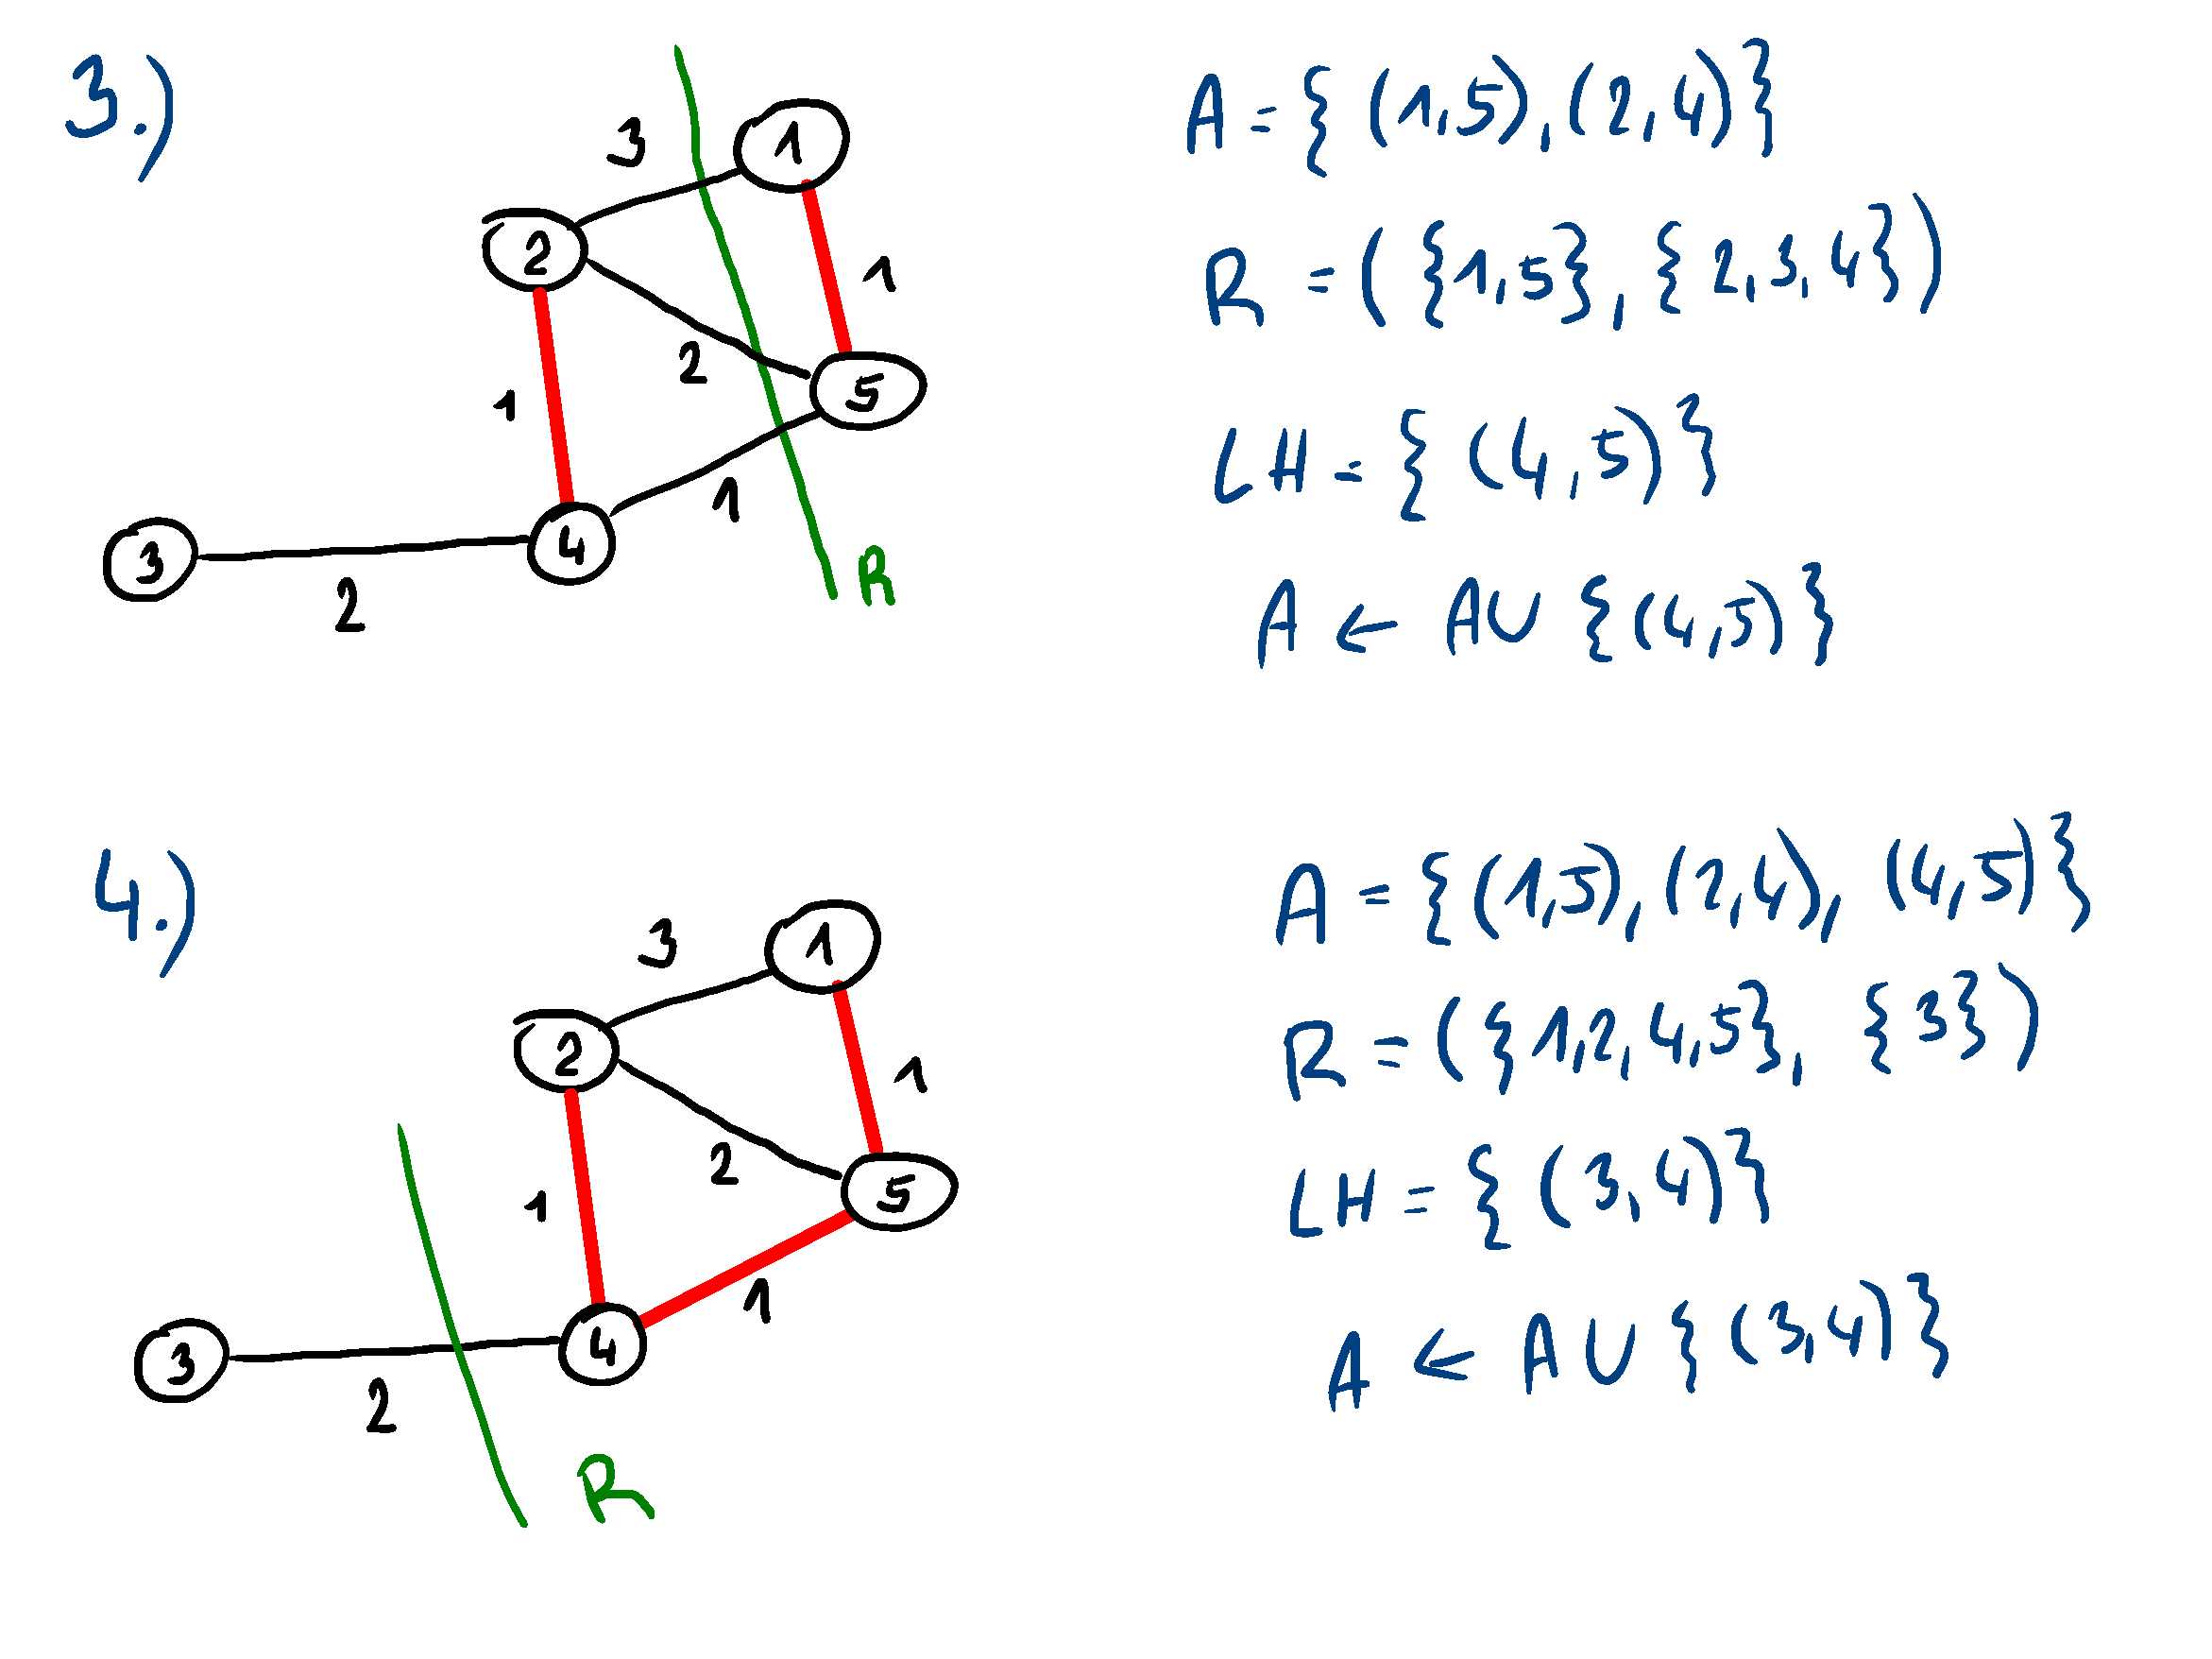
\includegraphics[width=0.9\linewidth]{03-minimalni-kostry-7.pdf}
    \caption{Příklad, část 2.}
\end{figure}

\begin{figure}[H]
    \centering
    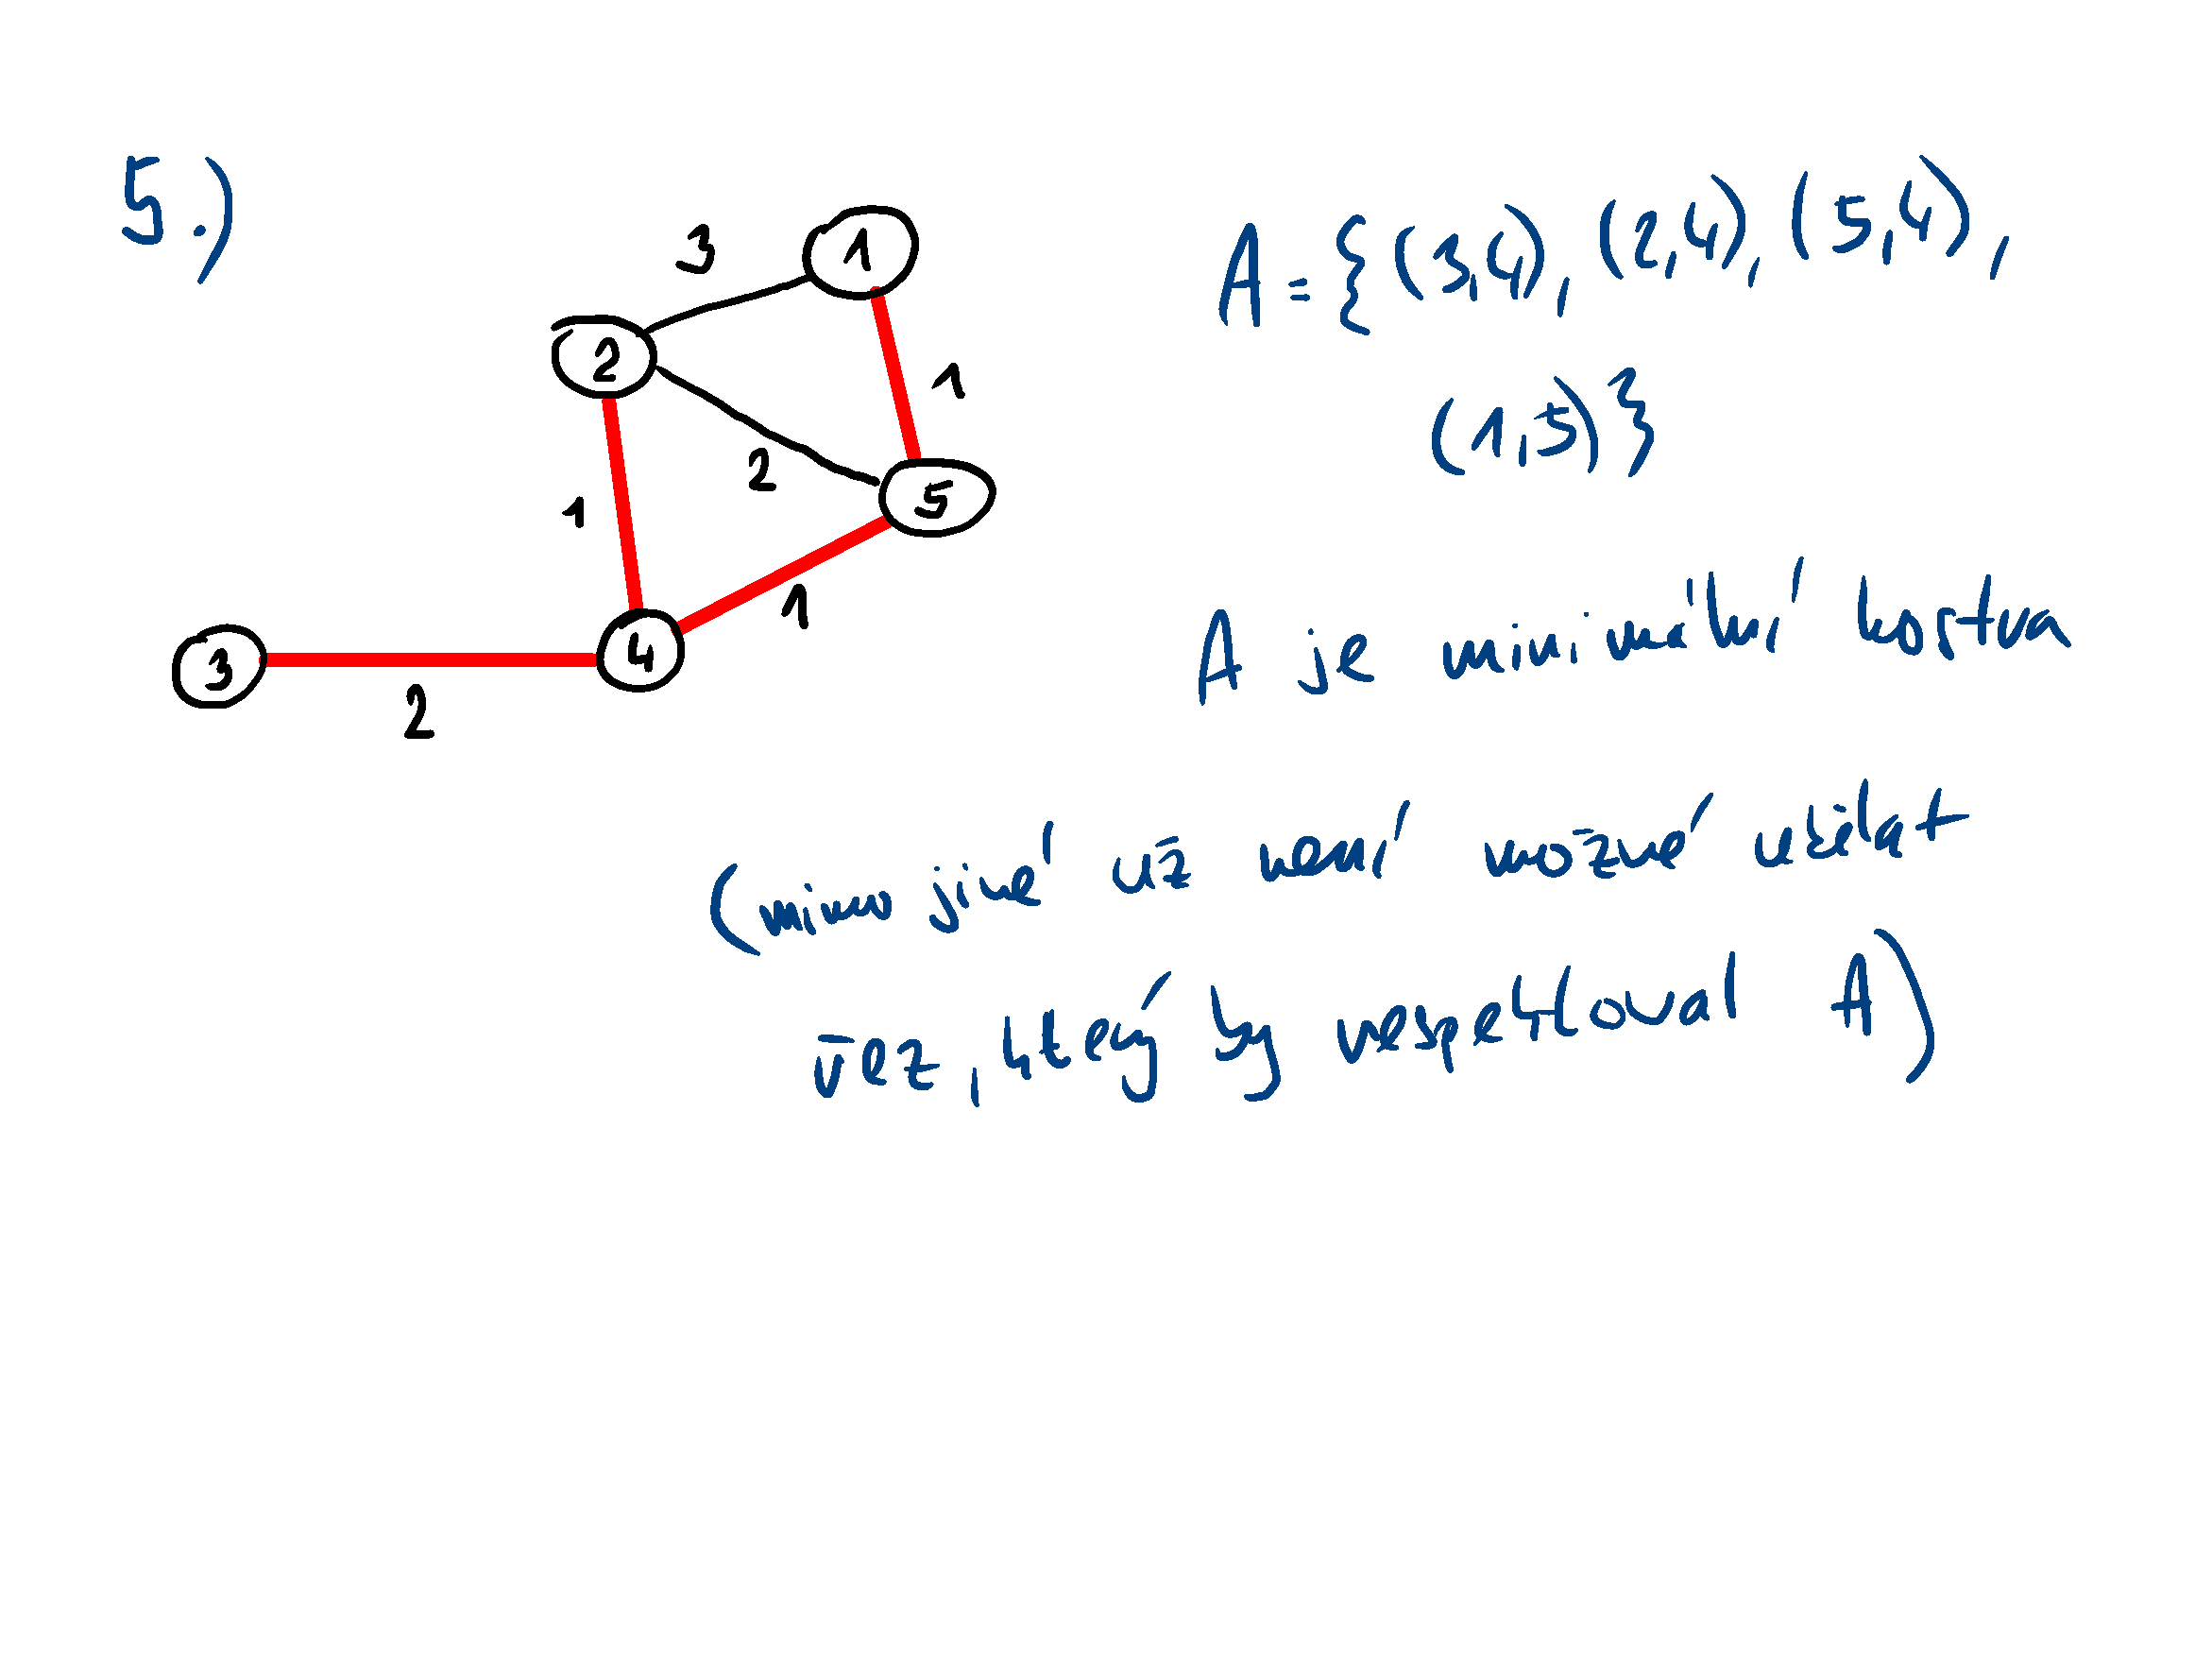
\includegraphics[width=0.9\linewidth]{03-minimalni-kostry-8.pdf}
    \caption{Příklad, část 3.}
\end{figure}

%%%%%%%%%%%%%%%%%%%%%%%%%%%%%%%%%%%%%%%%%%%%%%%%%%%%%%%%%%%%%%%%%%%%%%%%%%%%%%%%

\section{Kruskalův algoritmus}

Kruskalův a Primův algoritmus se liší v~tom, jakým způsobem vybírají bezpečnou hranu. Kruskalův algoritmus nahlíží na $A$ jako na les a hledá hranu s~nejmenším ohodnocením, která spojuje stromy v~lese. Na konci je $A$ jeden strom.

\bigskip\noindent\begin{minipage}{\linewidth}
\begin{lstlisting}[language=Python, caption={Kruskalův algoritmus. Funkce \texttt{make\_set(v)} vytvoří množinu obsahující $v$, \texttt{find\_set(v)} vrátí reprezentanta množiny ve které se nachází $v$, \texttt{union(u, v)} sjednotí dvě množiny obsahující $u$ a $v$.}]
def kruskal_mst(G):
    # G je graf

    # inicializace, kazdy uzel je ve sve mnozine
    A = {} # A je mnozina hran rozpracovane minimalni kostry
    for v in G.V:
        make_set(v)

    # seradit vzestupne podle w
    E = sort(G.E, G.w)

    for (u, v) in E:
        if find_set(u) != find_set(v):
            A += {(u, v)}
            union(u, v)

    return A
\end{lstlisting}
\end{minipage}

\subsection{Složitost}

\begin{compactitem}
    \item Řádek 5 -- $O(1)$
    \item Řádek 6-7 -- $n$-krát složitost $make\_set$ ($n$ je počet uzlů).
    \item Řádek 10 -- $O(m \cdot \log(m))$ ($m$ je počet hran).
    \item Řádky 12-15 -- Závisí na implementaci $find\_set$ a $union$.
    \begin{compactitem}
        \item Při implementaci seznamem s~heuristickou celkem: $O(m + n \cdot \log(n))$.
        \item Při stromové implementaci s~váhami a zkratkami celkem: $O((m+n) \cdot \alpha(n))$. Kde $\alpha$ je velmi pomalu rostoucí funkce ($\alpha \leq 4$).
    \end{compactitem}
    \item Pro souvislý graf platí $m > n$. Proto množinové operace stojí $O(m \cdot \alpha(n))$. Jelikož $\alpha(n) = O(\log(n)) = O(\log(m))$, tak celková složitost je $O(m \cdot \log(m))$.
    \item Dále platí $m < n^2$, pak $\log(m) = O(\log(n))$, proto celkem: $O(m \cdot \log(n))$.
\end{compactitem}

\subsection{Příklad}

\begin{figure}[H]
    \centering
    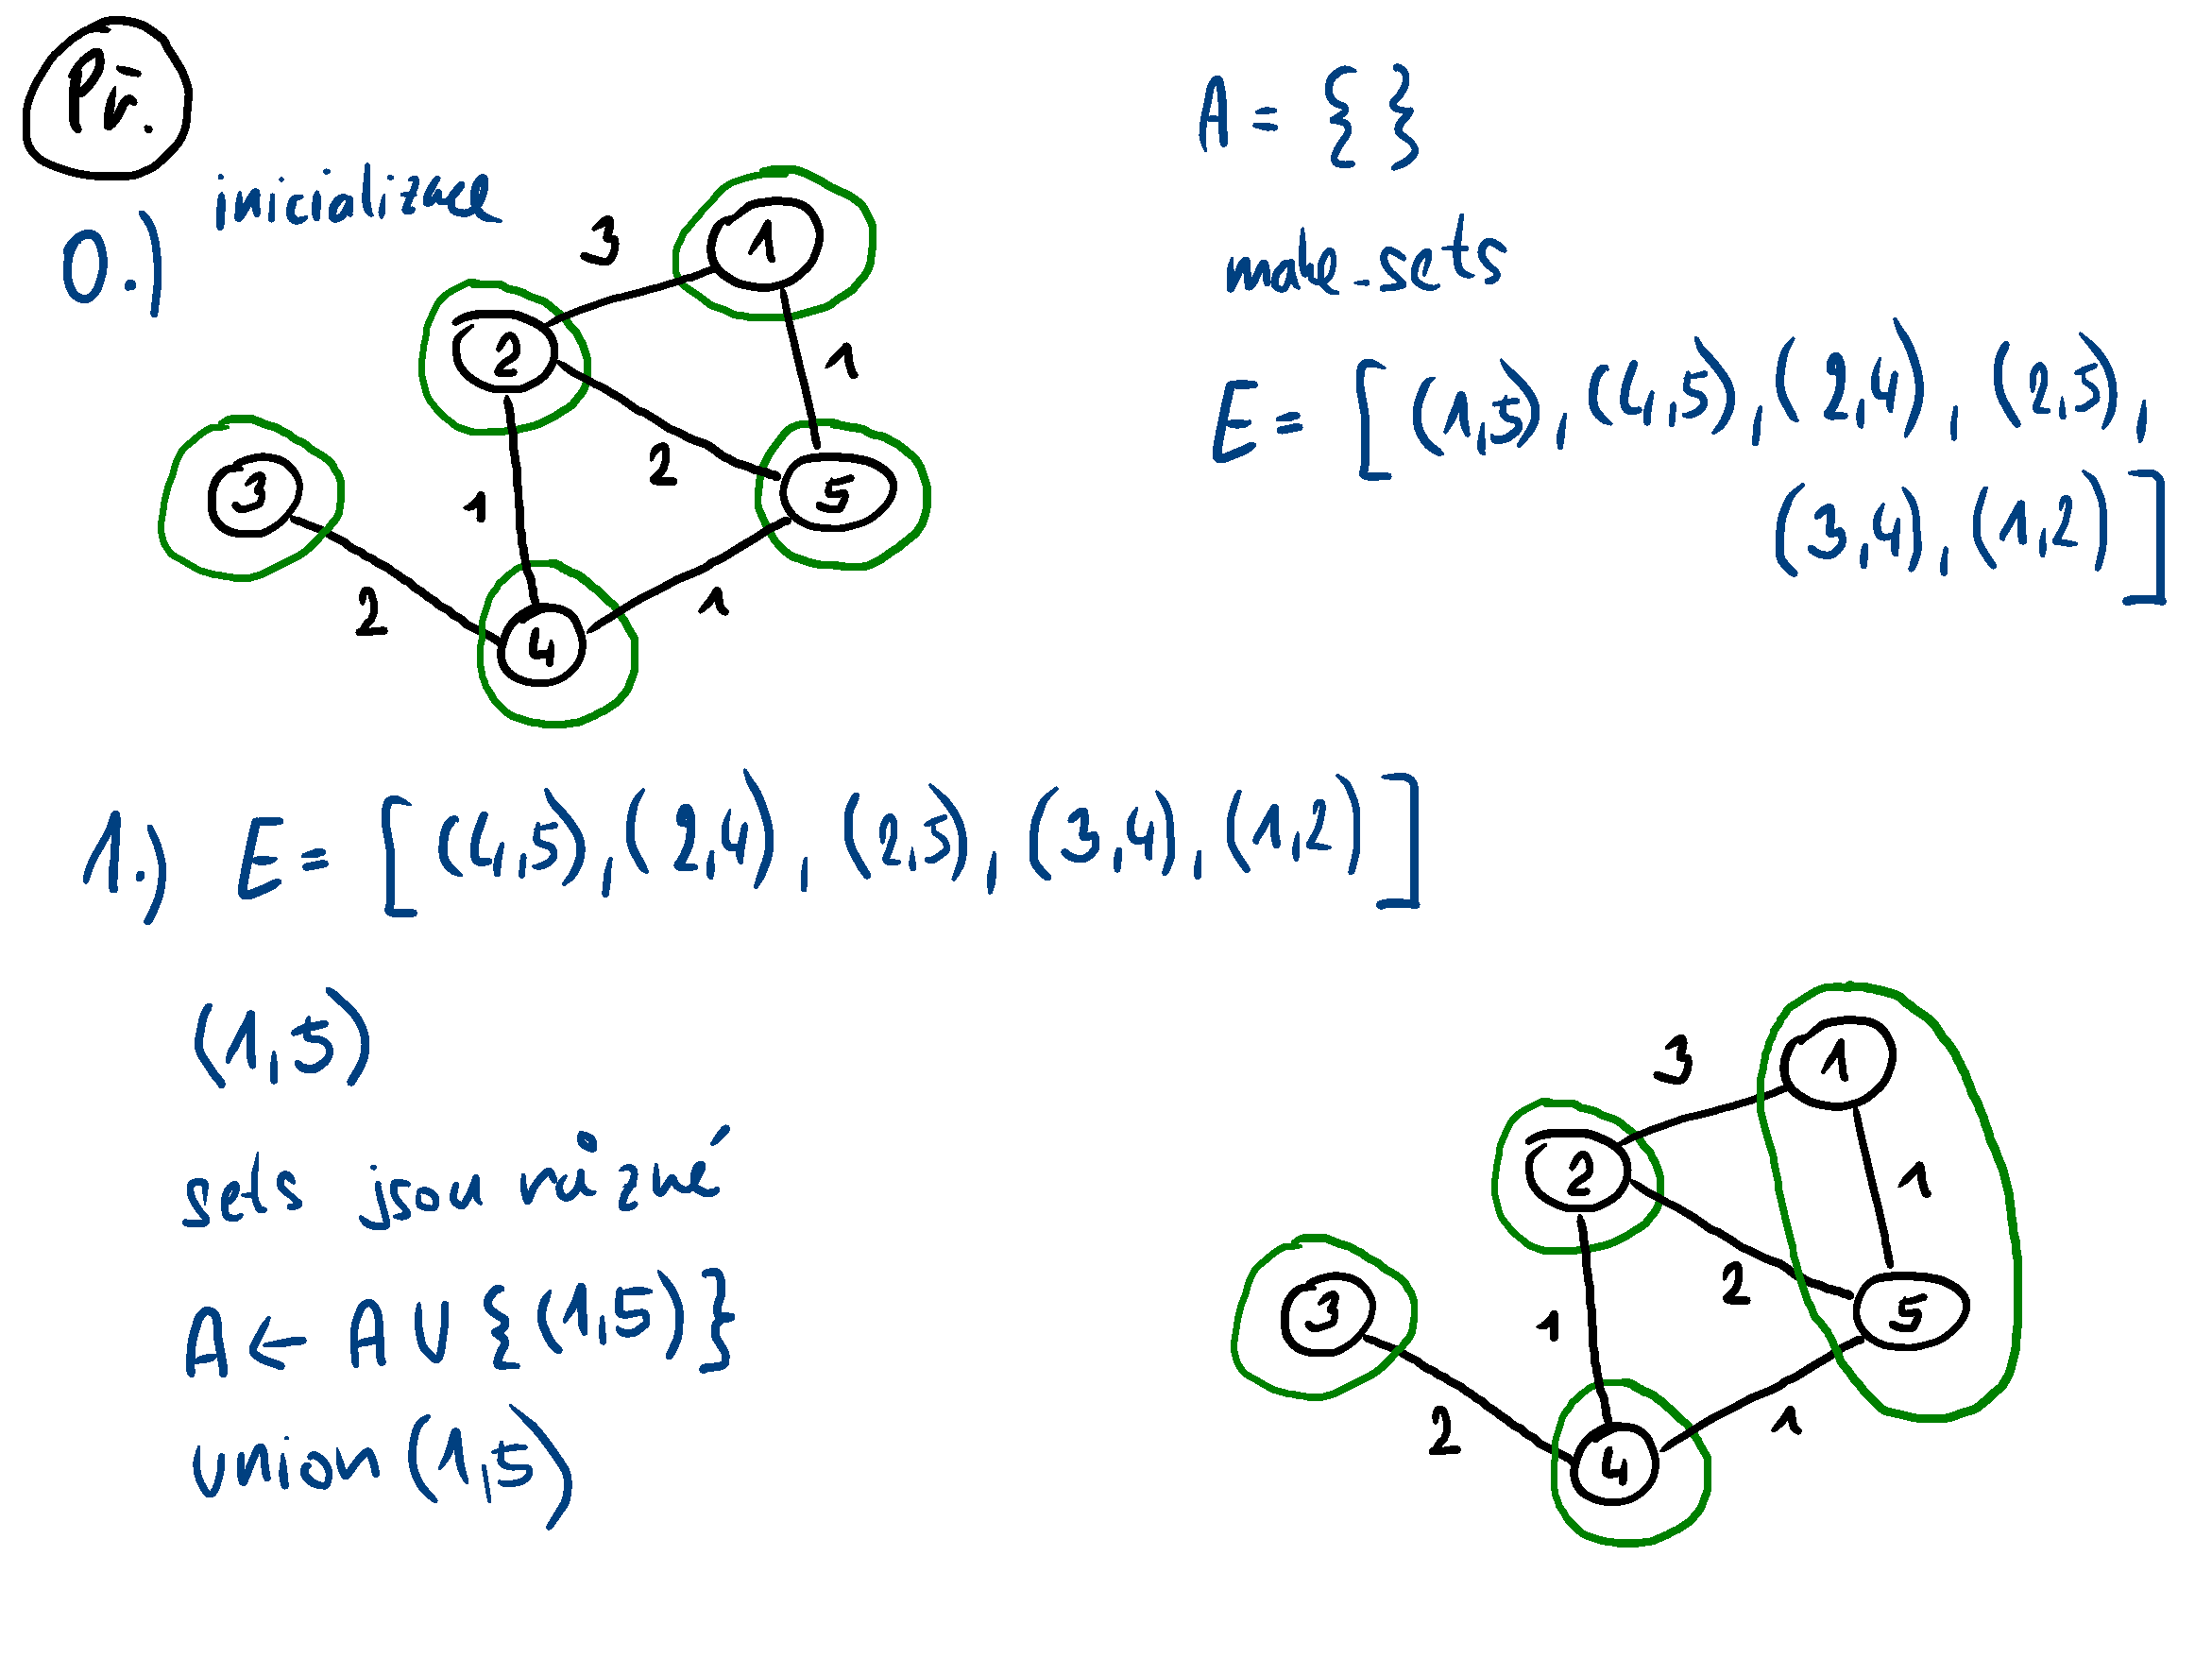
\includegraphics[width=0.9\linewidth]{03-minimalni-kostry-11.pdf}
    \caption{Příklad, část 1.}
\end{figure}

\begin{figure}[H]
    \centering
    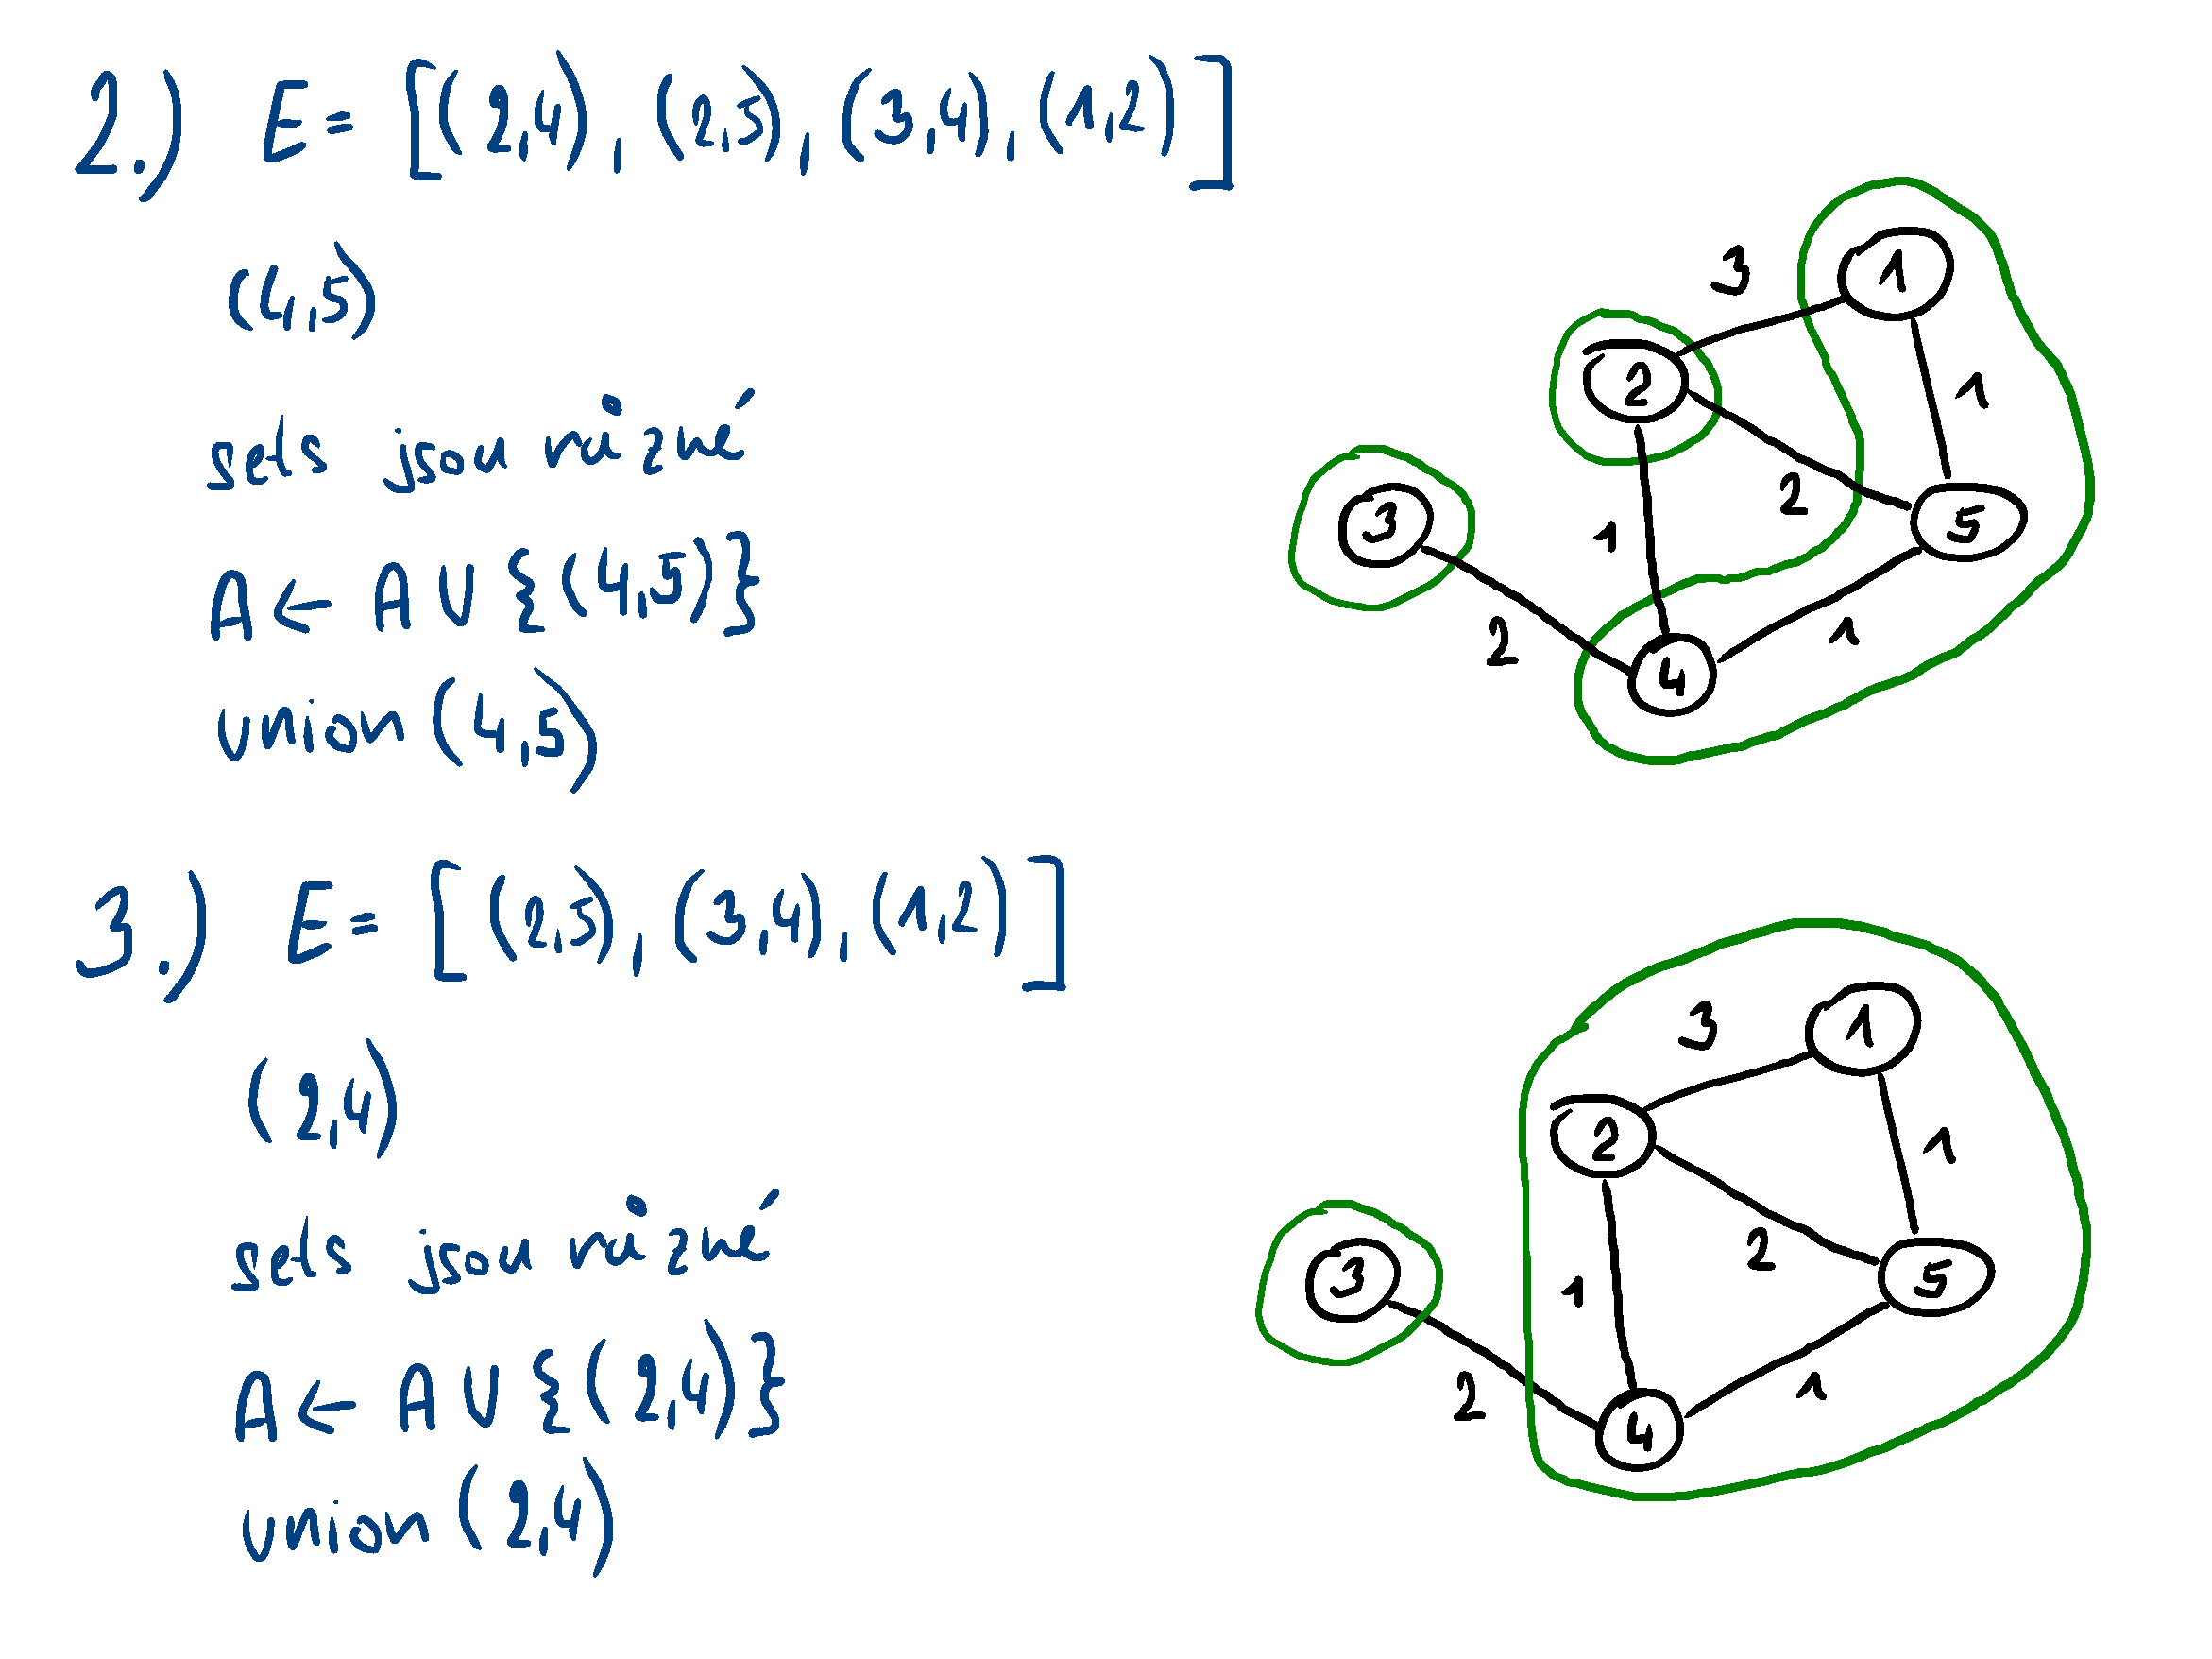
\includegraphics[width=0.9\linewidth]{03-minimalni-kostry-12.pdf}
    \caption{Příklad, část 2.}
\end{figure}

\begin{figure}[H]
    \centering
    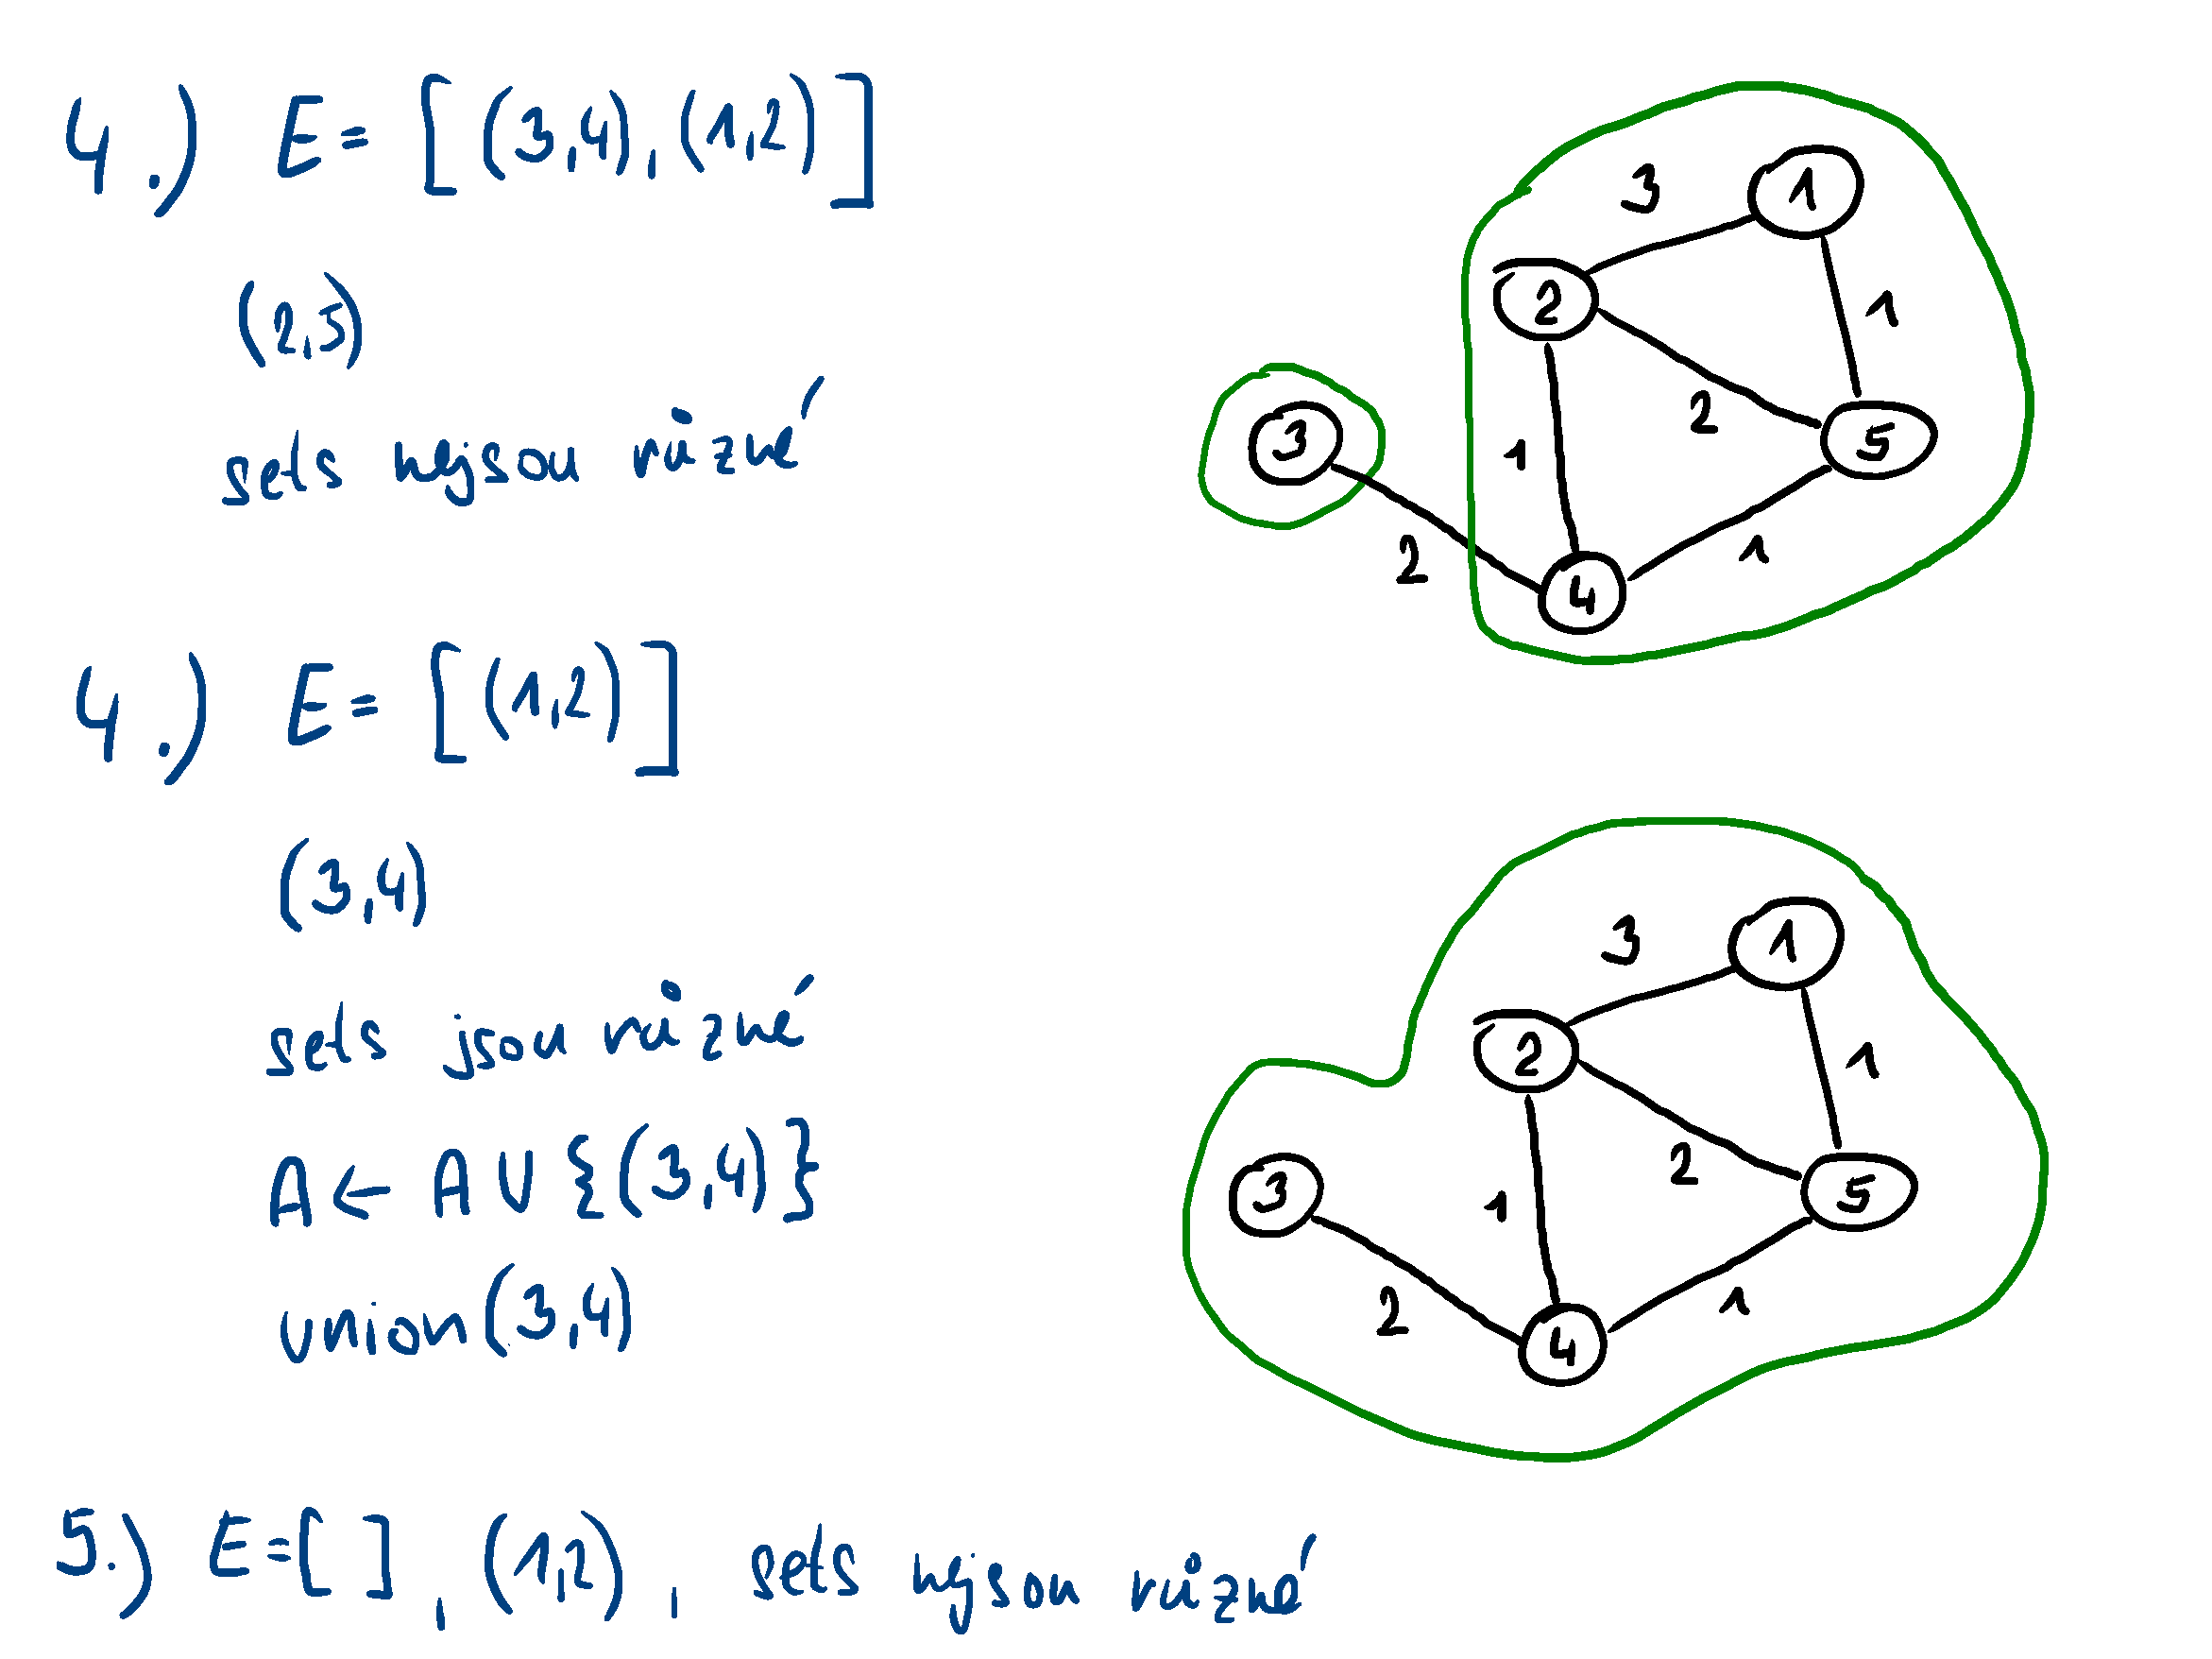
\includegraphics[width=0.9\linewidth]{03-minimalni-kostry-13.pdf}
    \caption{Příklad, část 3.}
\end{figure}

%%%%%%%%%%%%%%%%%%%%%%%%%%%%%%%%%%%%%%%%%%%%%%%%%%%%%%%%%%%%%%%%%%%%%%%%%%%%%%%%

\section{Primův-Jarníkův algoritmus}

Primův algoritmus buduje tzv. $A$ strom. Má zadaný určitý uzel, ze kterého hledá nejbližší další uzel, který by připojil. A~pak další a další.

\bigskip\noindent\begin{minipage}{\linewidth}
\begin{lstlisting}[language=Python, caption={Primův algoritmus.}]
def prim_mst(G, r):
    # G je graf
    # r je vychozi uzel

    for u in G.V:
        key[u] = INF # pole cen prechodu, kolik stoji prechod do vrcholu na indexu
        pi[u] = NULL # pole predchudcu, kdo je predchudce vrcholu na indexu

    key[r] = 0
    Q = Queue(G.V) # prioritni fronta uzlu

    while not Q.empty():
        u = Q.extract_min(key) # vrati prvek z Q s nejmensi hodnotou v key

        # pro vsechny sousedy uzlu u (Adj je seznam sousedu)
        for v in Adj[u]:
            # pokud je levnejsi cesta a jeste to neni prozkoumany uzel
            if v in Q and w(u, v) < key(v):
                pi[v] = u key[v] = w(u, v)
                Q.decrease_key(key) # aktualizace prioritni fronty

    return pi
\end{lstlisting}
\end{minipage}

\subsection{Složitost}

\begin{compactitem}
    \item Řádky 5-10 -- $O(n)$ za použití binární haldy ($n$ je počet uzlů).
    \item Řádky 12-13 -- While cyklus se provede n-krát a protože \textit{extract\_min} stojí $O(\log(n))$, tak je celková složitost $O(n \cdot \log(n))$.
    \item Řádek 16 -- For cyklus se provede $O(m)$ krát, protože dálka všech seznamů sousedů je dohromady $2m$ ($m$ je počet hran).
    \item Řádek 18-20 -- $O(1)$.
    \item Řádek 21 -- $O(\log(n))$.
    \item Jelikož $m > n$, tak celkem $O(n \cdot \log(n) + m \cdot \log(n)) = O(m \cdot \log(n))$.
\end{compactitem}

\subsection{Příklad}

\begin{figure}[H]
    \centering
    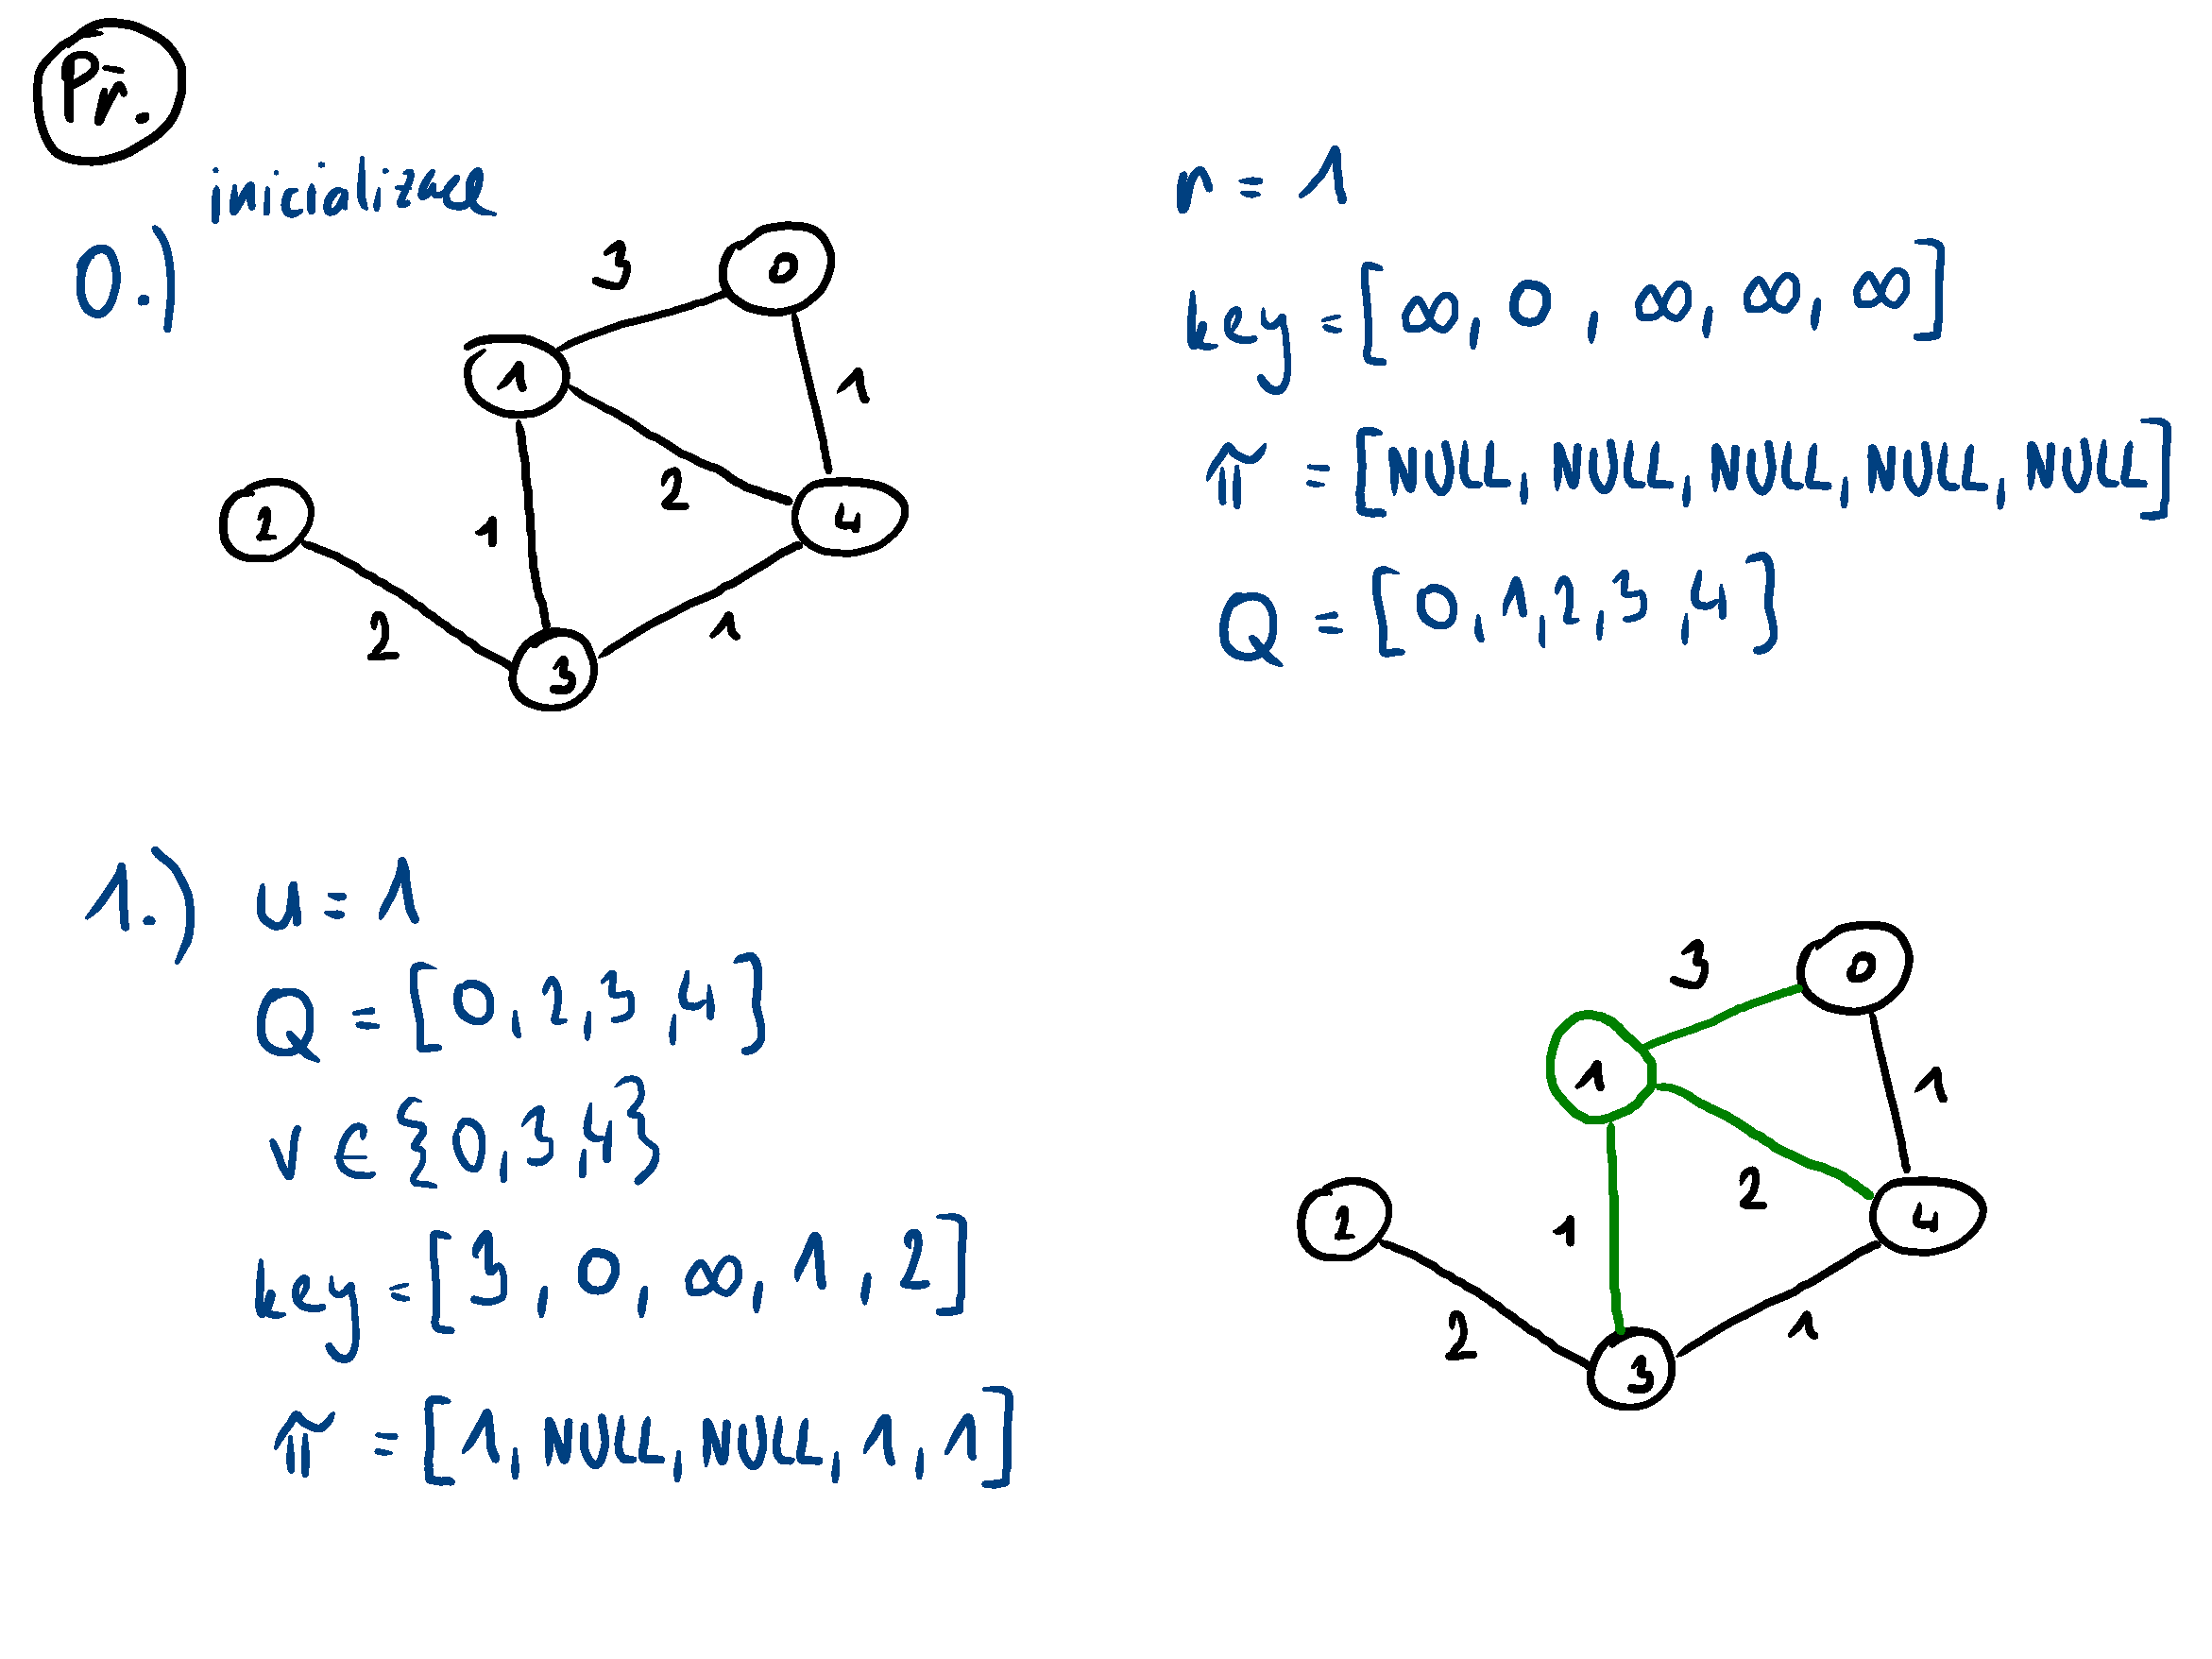
\includegraphics[width=0.9\linewidth]{03-minimalni-kostry-16.pdf}
    \caption{Příklad, část 1.}
\end{figure}

\begin{figure}[H]
    \centering
    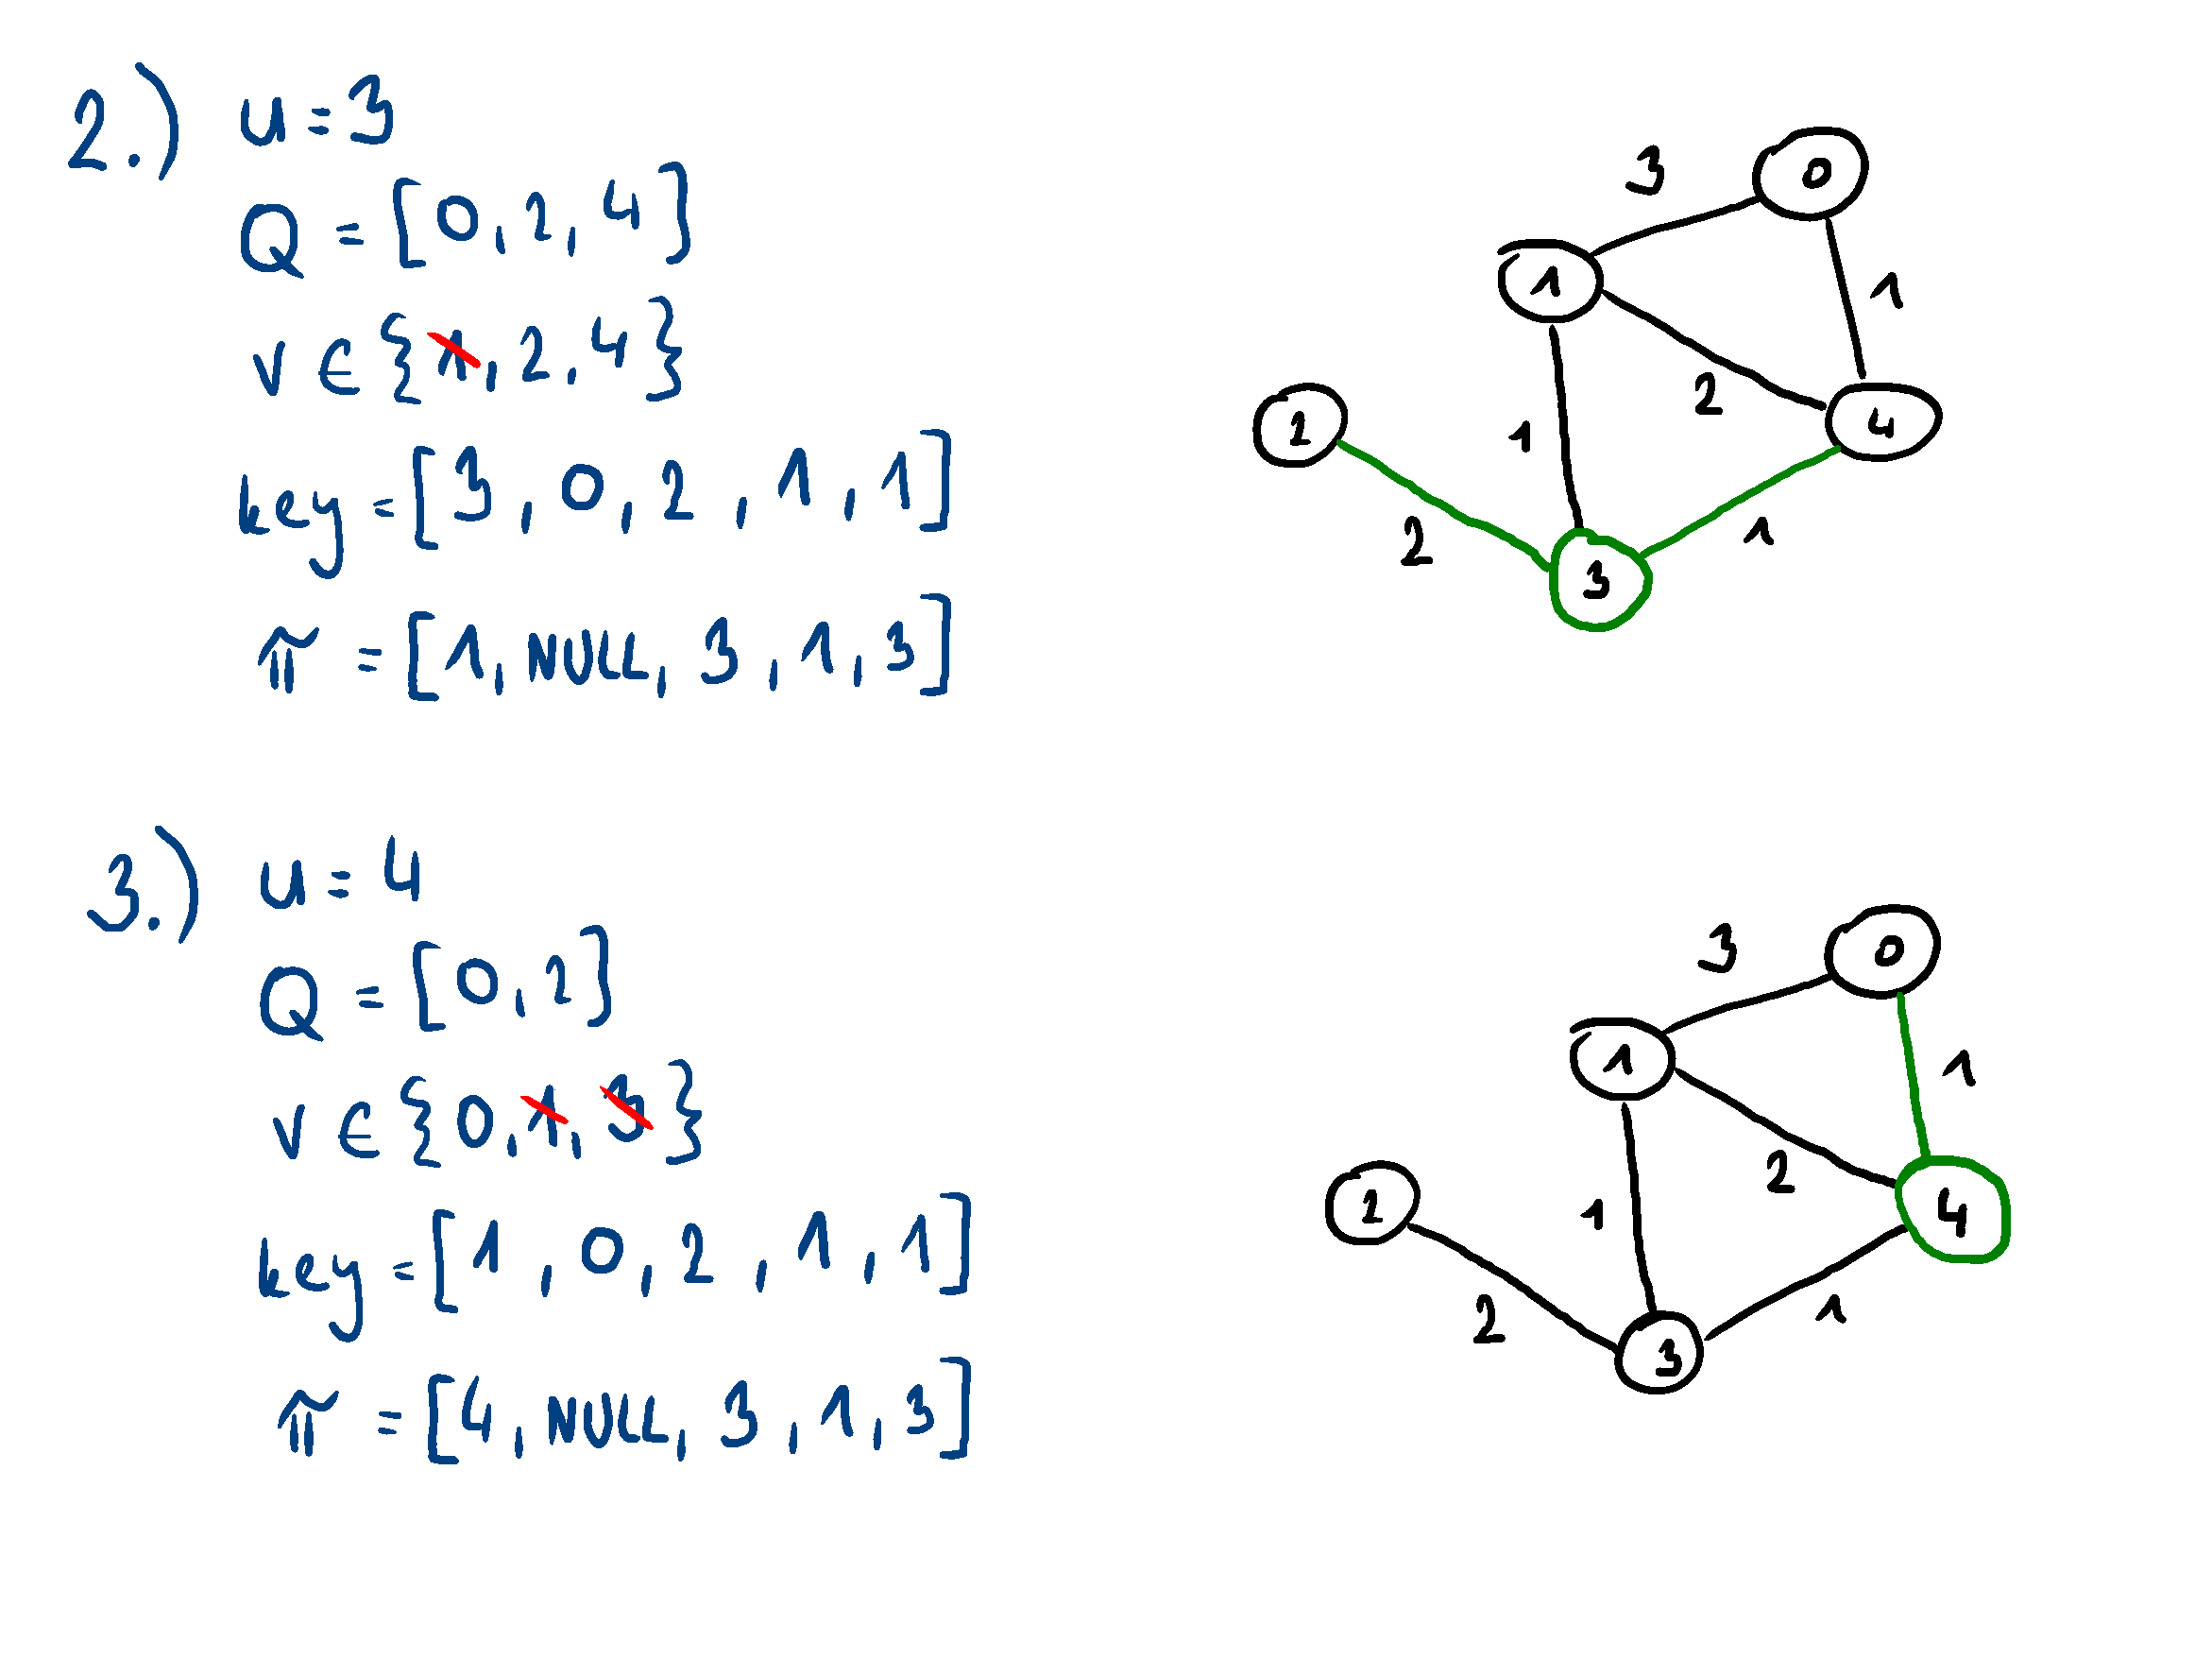
\includegraphics[width=0.9\linewidth]{03-minimalni-kostry-17.pdf}
    \caption{Příklad, část 2.}
\end{figure}

\begin{figure}[H]
    \centering
    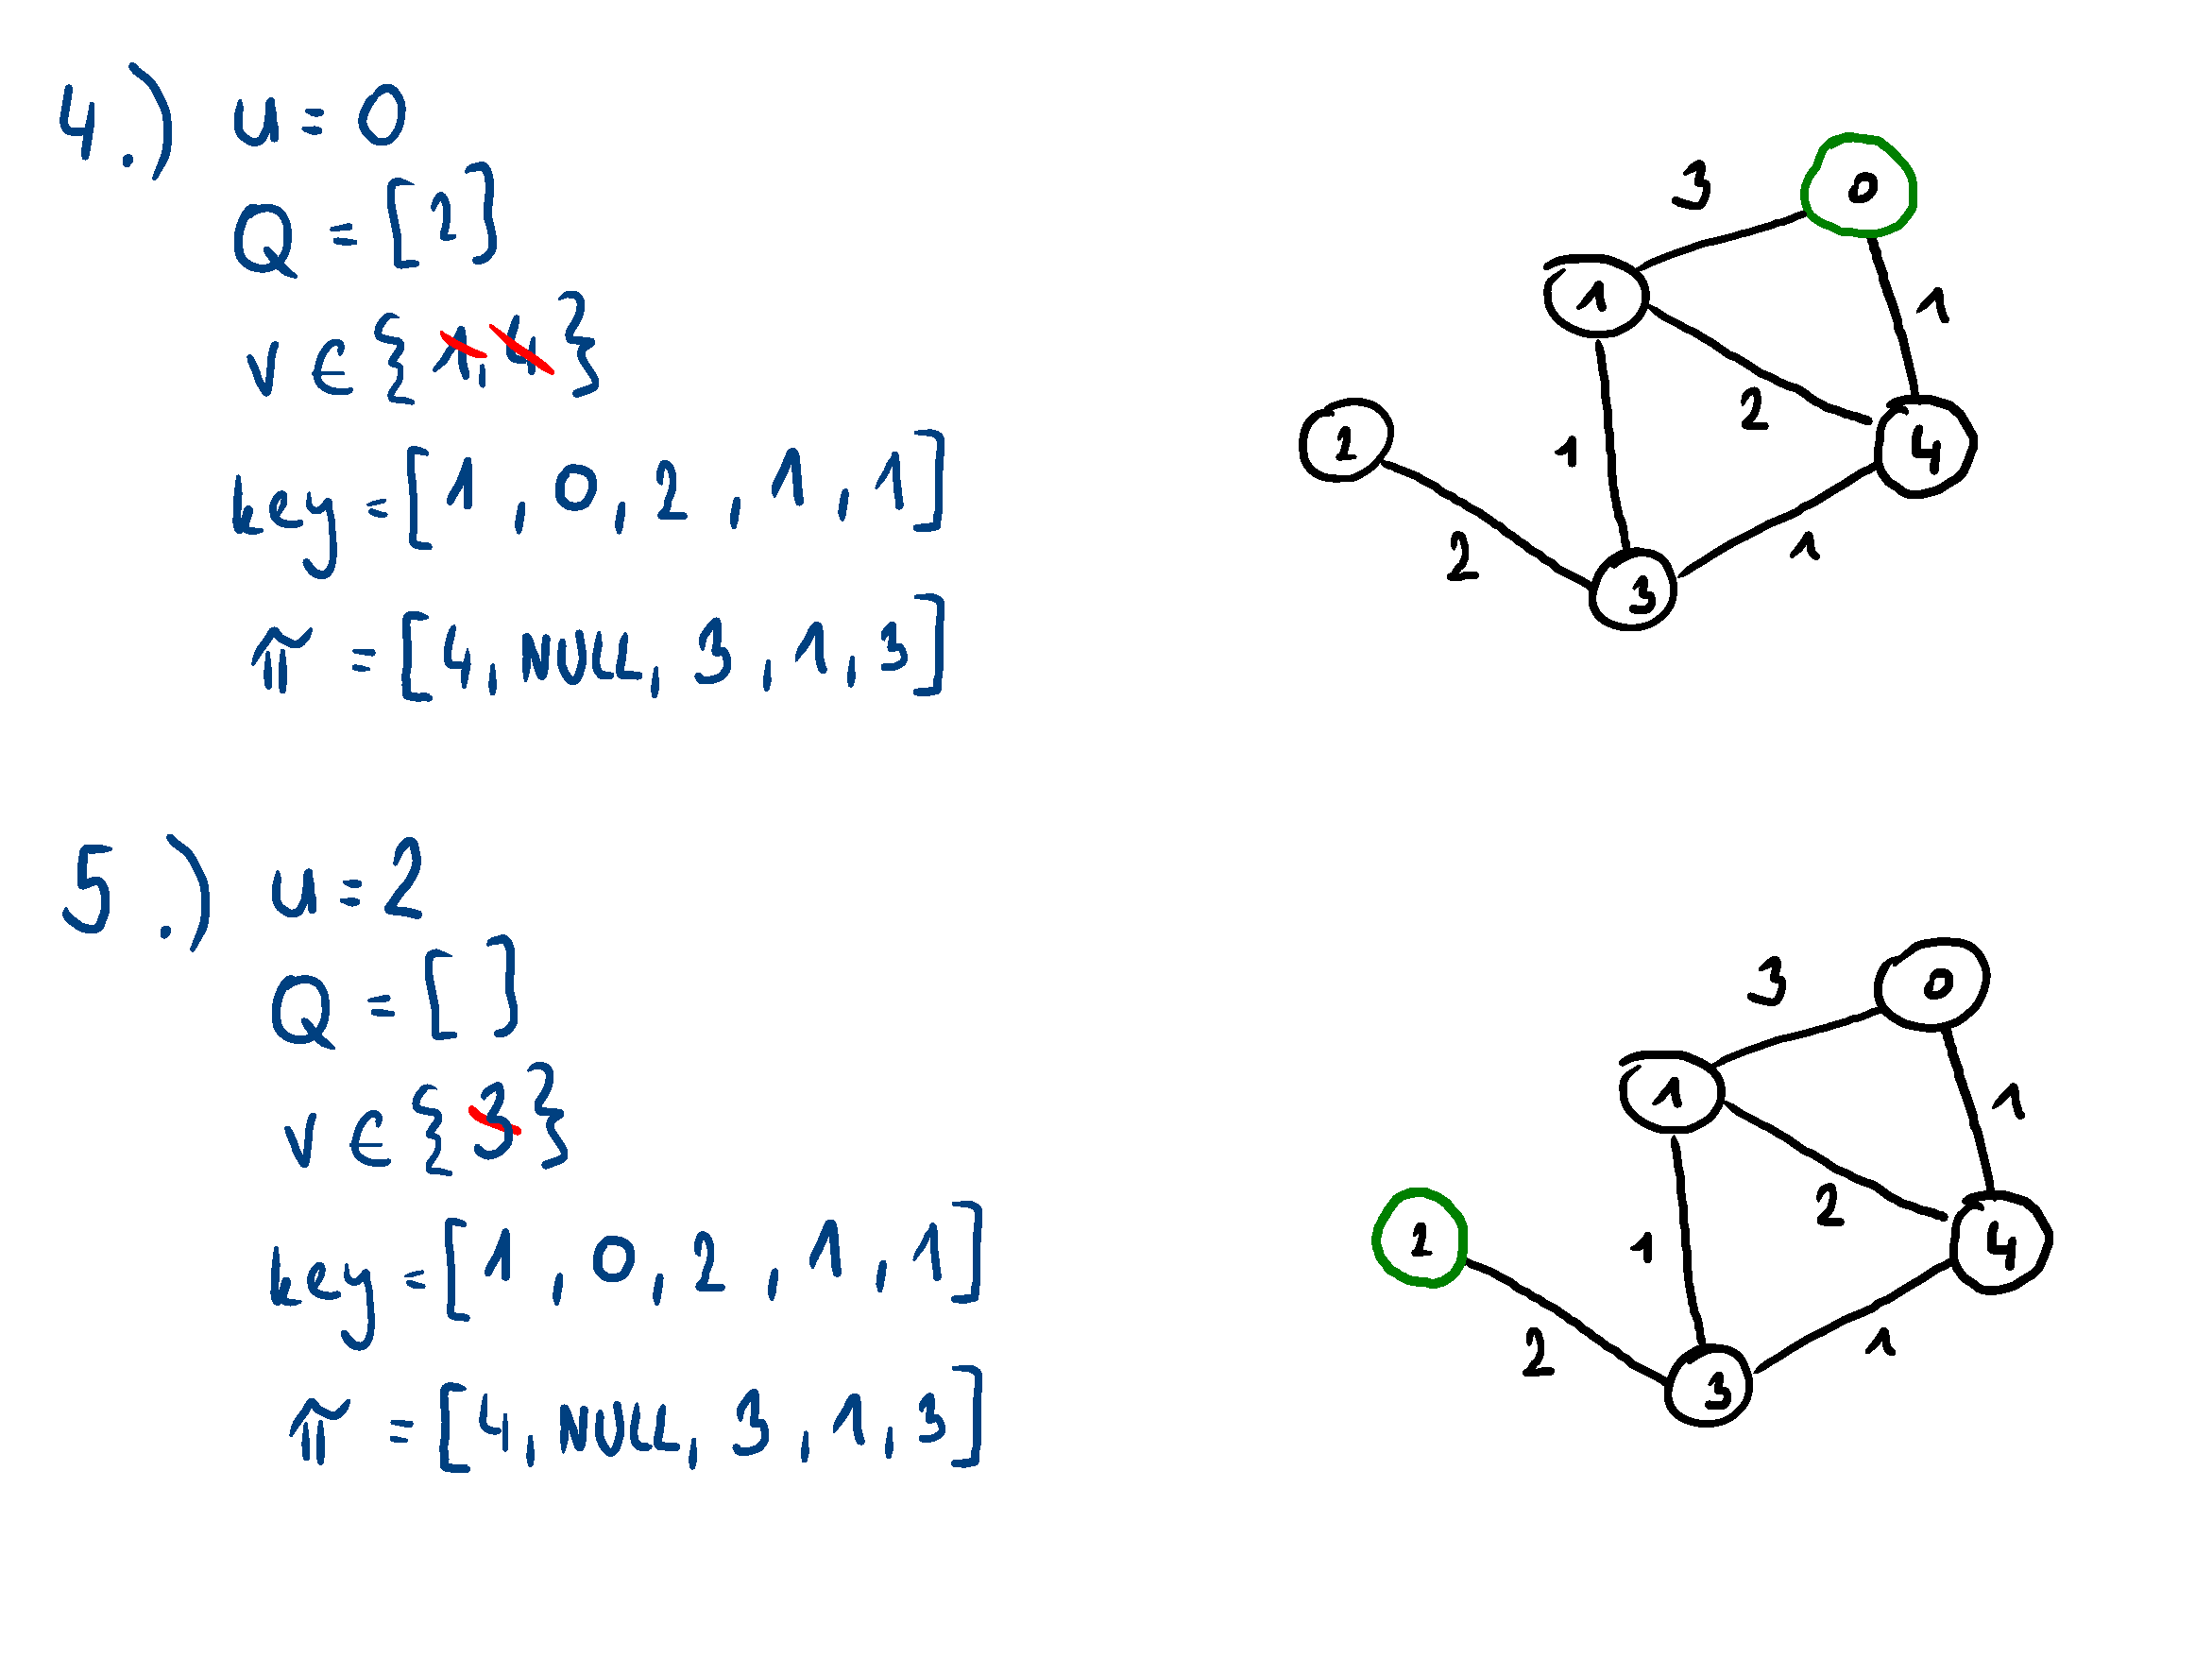
\includegraphics[width=0.9\linewidth]{03-minimalni-kostry-18.pdf}
    \caption{Příklad, část 3.}
\end{figure}

\begin{figure}[H]
    \centering
    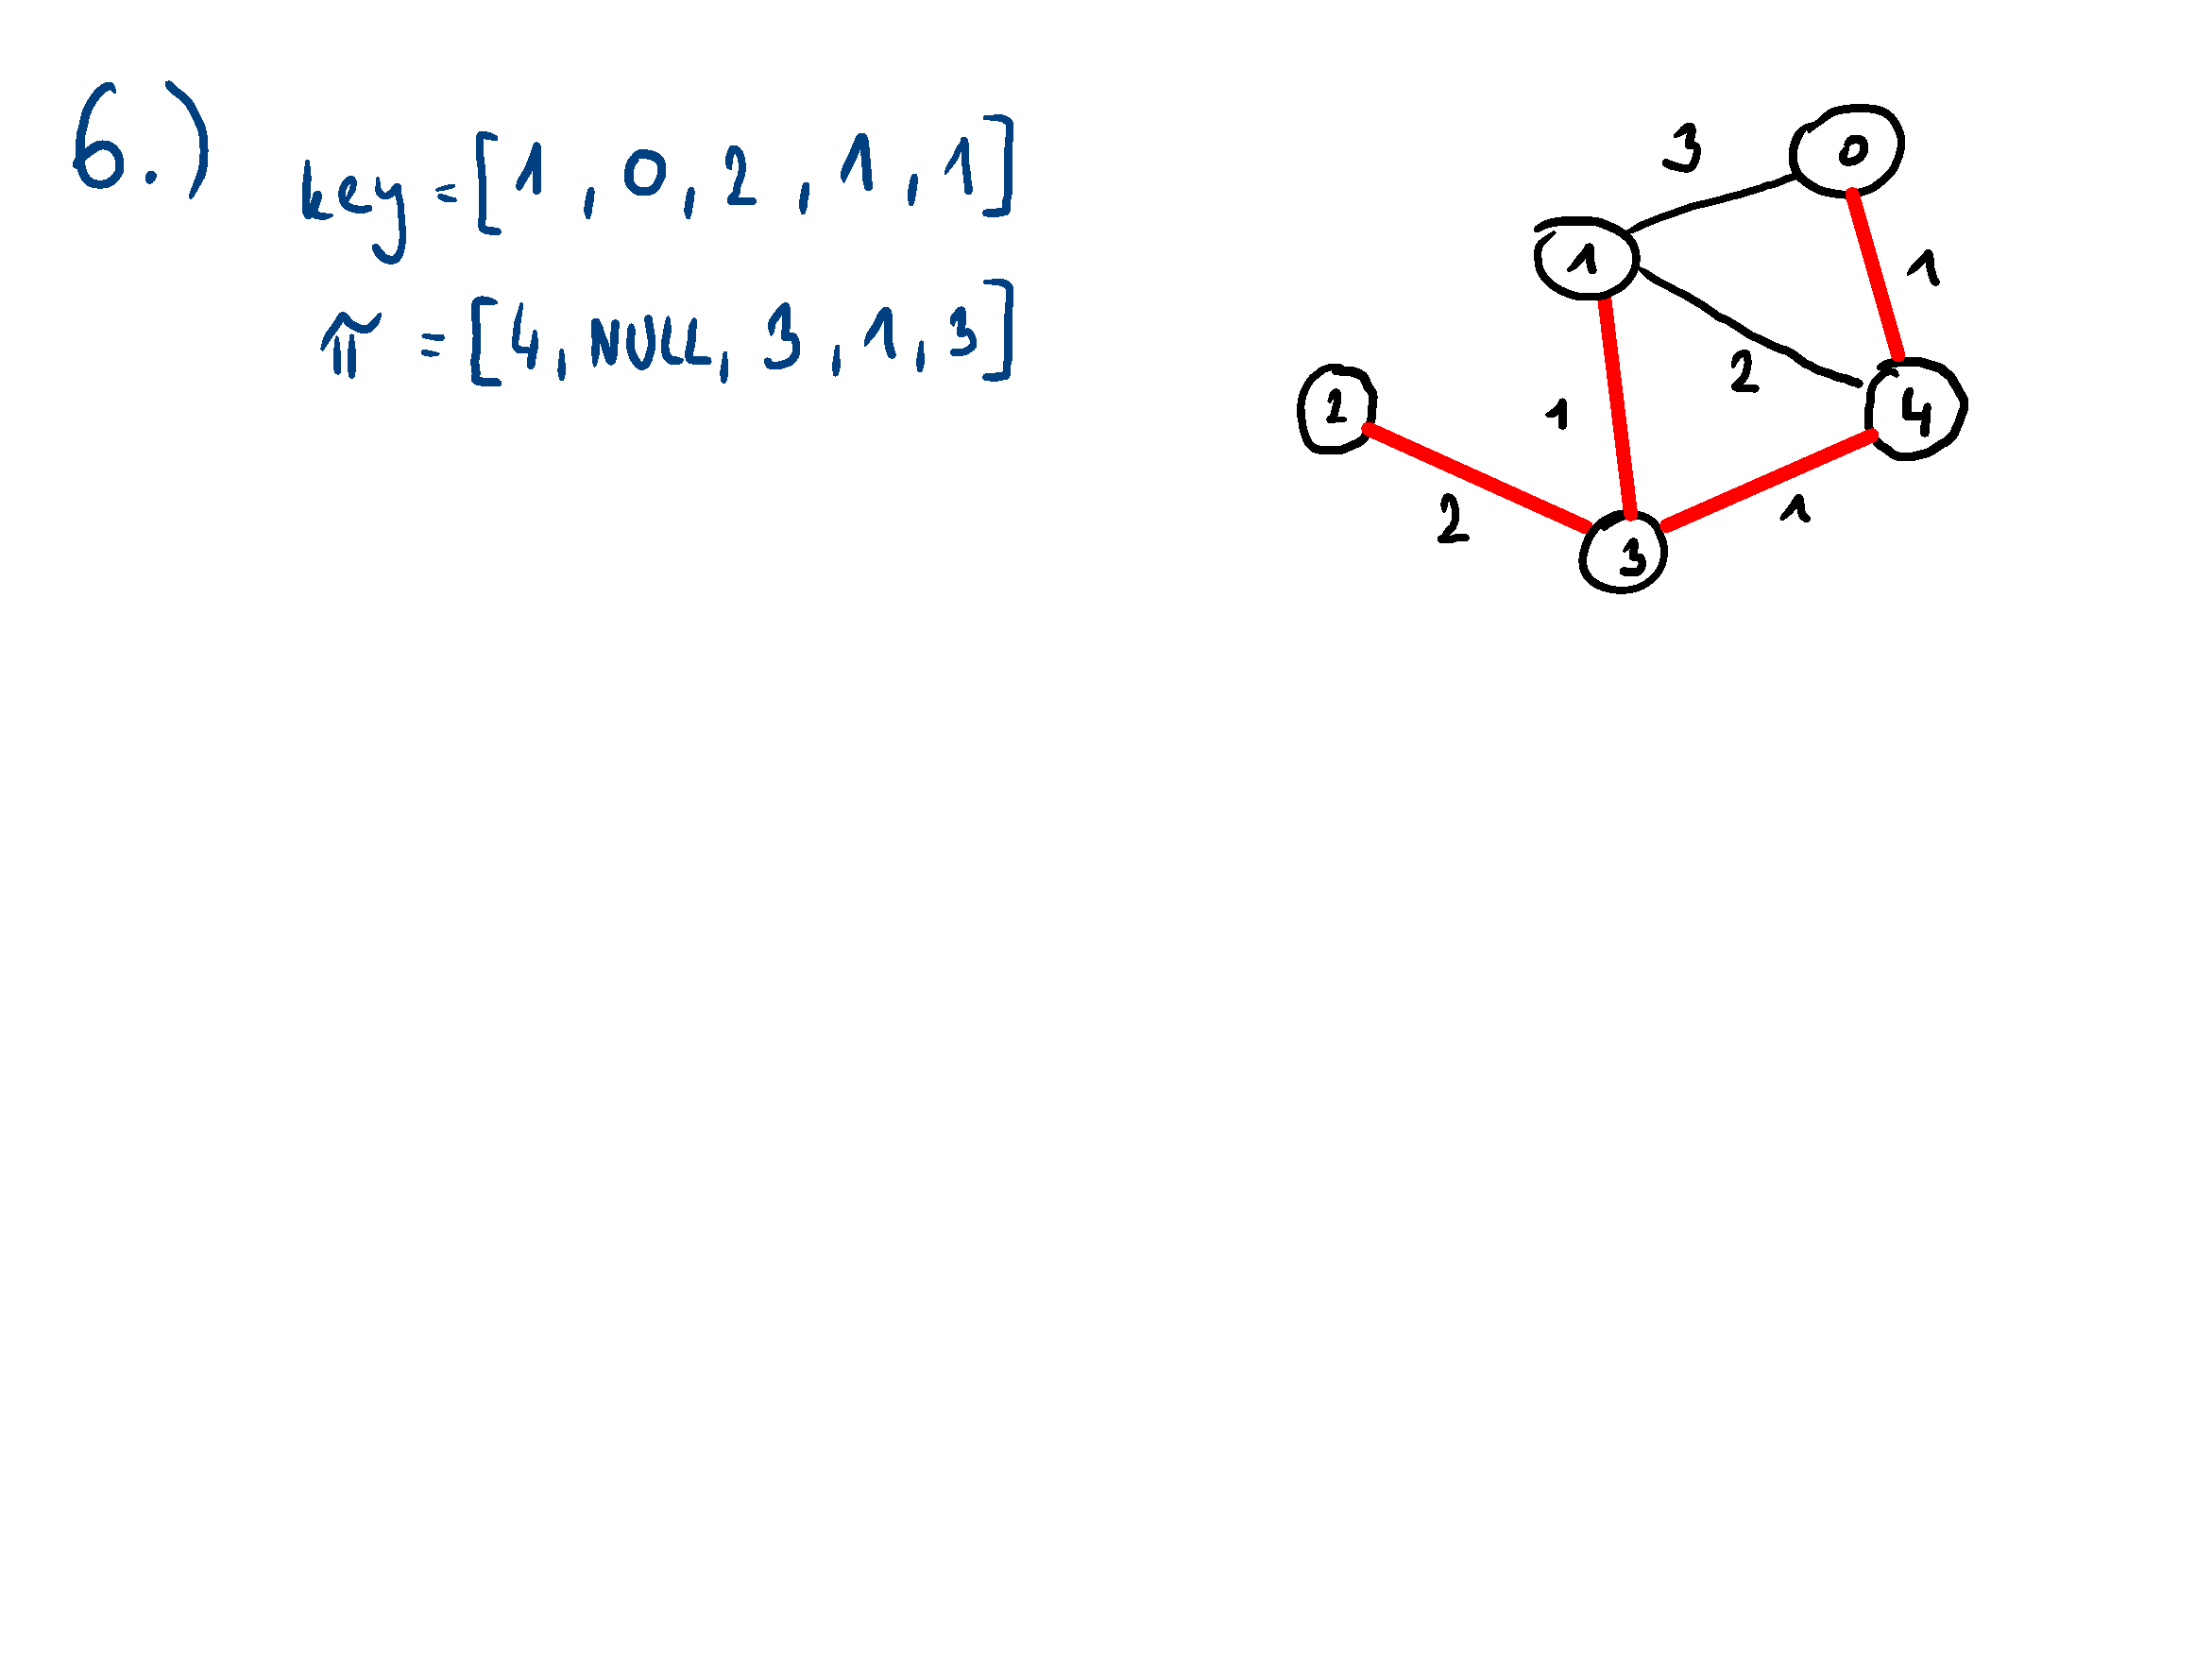
\includegraphics[width=0.9\linewidth]{03-minimalni-kostry-19.pdf}
    \caption{Příklad, část 4.}
\end{figure}
